\documentclass[a4paper,11pt]{article}
\usepackage[a4paper, top=2.5cm, bottom=2.5cm, left=2.2cm, right=2.2cm]{geometry}
\usepackage[T1]{fontenc}
\usepackage[utf8]{inputenc}
\usepackage{lmodern}
\usepackage{microtype}
\usepackage{graphicx}
\usepackage{booktabs}
\usepackage{longtable}
\usepackage[table]{xcolor}
\usepackage{colortbl}
\usepackage{titlesec}
\usepackage{fancyhdr}
\usepackage[hidelinks,
            pdftitle={XAI Project - Heart Failure Clinical Records},
            pdfauthor={Mattia Manneschi}]{hyperref}
\usepackage{caption}
\usepackage{float}
\usepackage{parskip}
\usepackage{array}
\usepackage{verbatim}

\definecolor{titlecol}{HTML}{1a1a2e}
\definecolor{accentcol}{HTML}{4C72B0}
\definecolor{tblhdr}{HTML}{4C72B0}
\definecolor{ltrow}{HTML}{f5f5f5}

\titleformat{\section}
  {\Large\bfseries\color{titlecol}}{\thesection}{0.8em}{}
  [{\color{accentcol}\hrule height 0.8pt\vspace{3pt}}]
\titleformat{\subsection}
  {\large\bfseries\color{titlecol}}{\thesubsection}{0.8em}{}
\titlespacing*{\section}{0pt}{18pt}{8pt}
\titlespacing*{\subsection}{0pt}{12pt}{4pt}

\pagestyle{fancy}
\fancyhf{}
\renewcommand{\headrulewidth}{0pt}
\fancyhead[L]{\small\color{gray}XAI Project --- Heart Failure Clinical Records}
\fancyhead[R]{\small\color{gray}\thepage}

\setlength{\parskip}{5pt}
\setlength{\parindent}{0pt}
\captionsetup{justification=raggedright,singlelinecheck=false}

\begin{document}

\begin{titlepage}
  \centering
  \vspace*{3cm}
  {\Huge\bfseries\color{titlecol} XAI Project\par}
  \vspace{0.8cm}
  {\LARGE\color{accentcol} Heart Failure Clinical Records\par}
  \vspace{0.6cm}
  {\large\color{gray}
    Confronto tra modelli interpretabili basati su regole\\[4pt]
    e modelli ensemble non interpretabili\par}
  \vspace{0.5cm}
  {\color{accentcol}\rule{\textwidth}{0.8pt}}
  \vspace{1.2cm}
  {\large Mattia Manneschi\par}
  \vspace{0.3cm}
  {\normalsize Laboratorio di Explainable AI\par}
  \vspace*{\fill}
\end{titlepage}

\tableofcontents
\clearpage

\section{Introduzione del problema e dataset}

\subsection{Contesto e motivazione}

\textbf{Il problema.}
L'insufficienza cardiaca è una condizione clinica grave in cui il cuore non riesce a pompare
sangue in modo sufficiente. Identificare i fattori di rischio associati al decesso è fondamentale
per supportare le decisioni cliniche e migliorare la prognosi dei pazienti.

\textbf{Obiettivo.}
Il progetto confronta due famiglie di modelli di machine learning per la predizione della
mortalità: modelli interpretabili basati su regole (rule-based) e modelli non interpretabili
basati su ensemble di alberi. L'obiettivo è valutare il trade-off tra performance predittiva e
interpretabilità in un contesto clinico ad alta criticità.

\textbf{Explainable AI in ambito clinico.}
In medicina, un modello non spiegabile --- per quanto accurato --- non è direttamente utilizzabile
come strumento di supporto decisionale: il medico deve poter comprendere e validare le motivazioni
di ogni predizione. I modelli intrinsecamente interpretabili soddisfano questo requisito senza
richiedere metodi post-hoc aggiuntivi (es.\ SHAP, LIME), che possono introdurre approssimazioni
e spiegazioni fuorvianti.

\textbf{Struttura del report.}
Il Capitolo~1 introduce il problema clinico, descrive il dataset e presenta l'analisi esplorativa.
Il Capitolo~2 illustra l'architettura del progetto, la pipeline di elaborazione dei dati, i modelli
utilizzati e la loro configurazione. Il Capitolo~3 presenta i risultati e il confronto delle
performance. Il Capitolo~4 raccoglie le conclusioni, l'analisi clinica dei risultati e i limiti
del lavoro.

\clearpage
\subsection{Il Dataset}

Il dataset \emph{Heart Failure Clinical Records} (UCI, id=519) raccoglie cartelle cliniche di
299 pazienti con insufficienza cardiaca seguiti in follow-up. La variabile target
\texttt{DEATH\_EVENT} indica se il paziente è deceduto durante il periodo di osservazione.

\medskip
\noindent Campioni: 299 $\;|\;$ Decessi: 96 (32.1\%) $\;|\;$ Sopravvissuti: 203 (67.9\%)

\medskip
\textbf{Gestione delle feature: binarie vs continue.}
Le 12 feature si dividono in 5 binarie (\texttt{anaemia}, \texttt{diabetes},
\texttt{high\_blood\_pressure}, \texttt{sex}, \texttt{smoking}) e 7 continue.
I modelli ensemble e la maggior parte dei rule-based le ricevono direttamente.
RuleFit richiede standardizzazione (StandardScaler), mentre BayesianRuleList richiede feature
esclusivamente binarie: le variabili continue vengono discretizzate in bin tramite
KBinsDiscretizer (one-hot, 4 bin quantili) prima del fitting.

\medskip
\begin{center}
{\small\begin{tabular}{>{\raggedright\arraybackslash}p{0.2375\linewidth}>{\raggedright\arraybackslash}p{0.1096\linewidth}>{\raggedright\arraybackslash}p{0.5664\linewidth}}
\toprule
\cellcolor{tblhdr}\color{white}\bfseries Feature & \cellcolor{tblhdr}\color{white}\bfseries Tipo & \cellcolor{tblhdr}\color{white}\bfseries Descrizione \\
\midrule
age & continua & Eta' del paziente (anni) \\
\rowcolor{ltrow}anaemia & binaria & Presenza di anemia (0/1) \\
creatinine\_\allowbreak{}phosphokinase & continua & Livello CPK nel sangue (mcg/L) \\
\rowcolor{ltrow}diabetes & binaria & Presenza di diabete (0/1) \\
ejection\_\allowbreak{}fraction & continua & Percentuale di sangue pompata dal ventricolo sinistro (\%) \\
\rowcolor{ltrow}high\_\allowbreak{}blood\_\allowbreak{}pressure & binaria & Presenza di ipertensione (0/1) \\
platelets & continua & Conta piastrinica (kiloplatelets/mL) \\
\rowcolor{ltrow}serum\_\allowbreak{}creatinine & continua & Livello di creatinina serica (mg/dL) \\
serum\_\allowbreak{}sodium & continua & Livello di sodio sierico (mEq/L) \\
\rowcolor{ltrow}sex & binaria & Sesso biologico (0=F, 1=M) \\
smoking & binaria & Fumatore (0/1) \\
\rowcolor{ltrow}time & continua & Durata del follow-up (giorni) \\
\bottomrule
\end{tabular}}}
\end{center}

\clearpage
\subsection{EDA --- Distribuzioni per classe}

\begin{figure}[H]
  \centering
  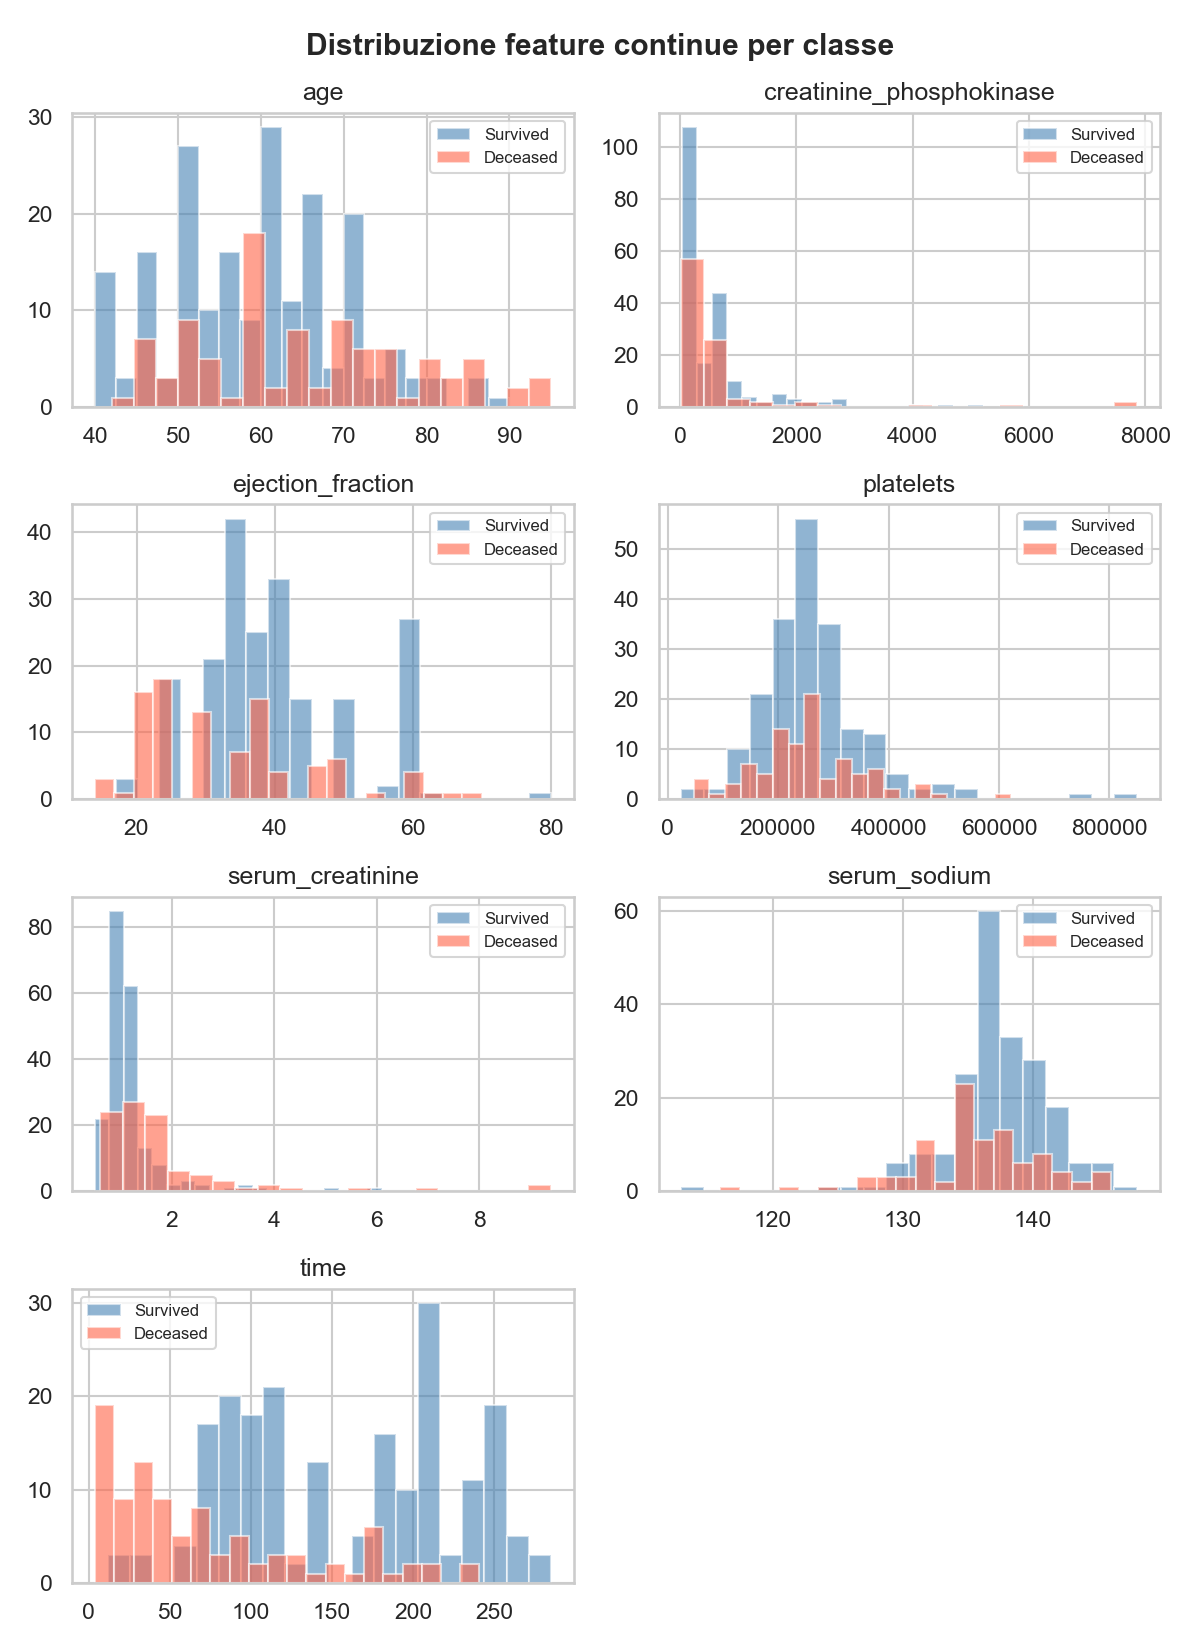
\includegraphics[width=\textwidth]{figures/eda_continuous.png}
\end{figure}

Ogni istogramma sovrappone la distribuzione di una feature per sopravvissuti (blu) e deceduti
(rosso). \texttt{time} è il discriminatore più potente: un follow-up breve corrisponde quasi
sempre a decesso. \texttt{serum\_creatinine} alta indica compromissione renale; \texttt{ejection\_fraction}
bassa segnala ridotta capacità di pompa. \texttt{platelets} e \texttt{creatinine\_phosphokinase}
mostrano distribuzioni largamente sovrapposte.

\clearpage
\subsection{EDA --- Matrice di correlazione}

\begin{figure}[H]
  \centering
  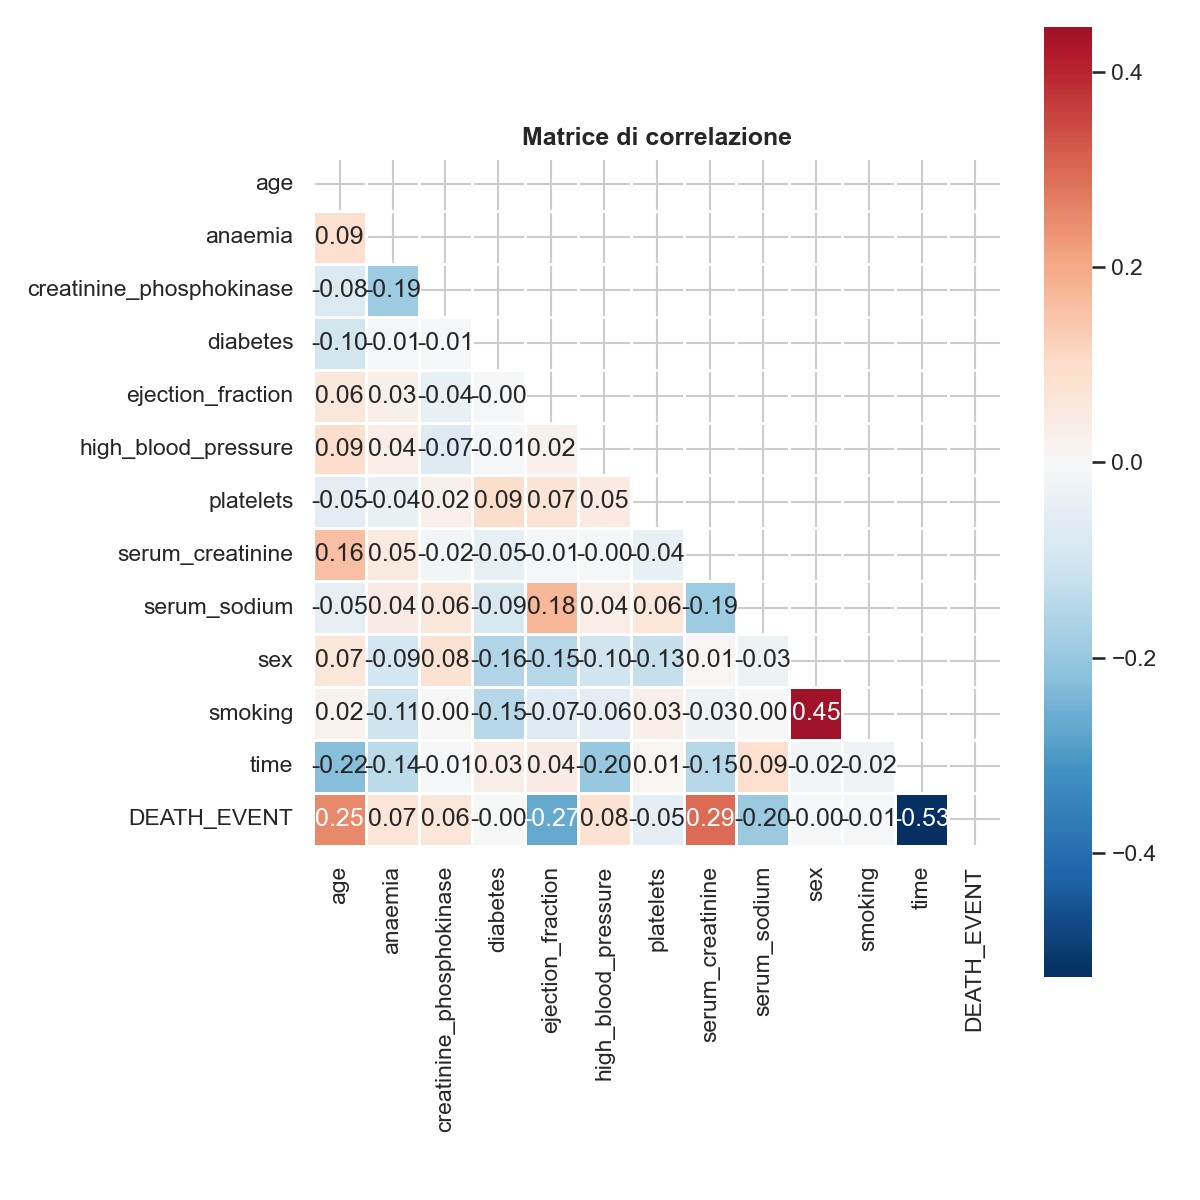
\includegraphics[width=\textwidth]{figures/eda_correlation.png}
\end{figure}

\texttt{time} ha la correlazione più forte con DEATH\_EVENT ($-$0.53): pazienti con follow-up
lungo tendono a sopravvivere. \texttt{serum\_creatinine} (+0.29) ed
\texttt{ejection\_fraction} ($-$0.27) sono i segnali biochimici più informativi.
Le feature binarie mostrano correlazioni deboli ($< \pm 0.15$).


\section{Architettura e Implementazione}

\subsection{Struttura del Progetto}

Il progetto è organizzato in una cartella \texttt{src/} con sette moduli distinti, ciascuno
con una responsabilità precisa. Questa separazione permette di modificare una componente senza
toccare le altre e rende il codice più leggibile e testabile.

\medskip
\begin{center}
{\small\begin{tabular}{>{\raggedright\arraybackslash}p{0.2066\linewidth}>{\raggedright\arraybackslash}p{0.7325\linewidth}}
\toprule
\cellcolor{tblhdr}\color{white}\bfseries Modulo & \cellcolor{tblhdr}\color{white}\bfseries Responsabilita' \\
\midrule
config.py & Centralizza iperparametri, path e costanti \\
\rowcolor{ltrow}data\textbackslash{}\_loader.py & Download UCI, cache CSV, split stratificato 60/20/20, tre varianti di preprocessing \\
models.py & Factory function per ciascuno dei 9 modelli; accetta **params per override \\
\rowcolor{ltrow}evaluate.py & Calcolo metriche, generazione di tutti i grafici, cross-validation \\
tune.py & Grid search esaustiva sul validation set (ROC-AUC) \\
\rowcolor{ltrow}main.py & Orchestrazione dell'intera pipeline end-to-end \\
report\textbackslash{}\_latex.py & Legge gli artefatti salvati e genera il report LaTeX/PDF \\
\bottomrule
\end{tabular}}}
\end{center}

\medskip
\textbf{Output della pipeline.}
Ogni esecuzione di \texttt{main.py} produce artefatti su disco: i dati grezzi vengono cachati
in \texttt{data/}; le metriche e le regole vengono salvate in \texttt{results/files/}; i
grafici in \texttt{results/plots/}; il report finale in \texttt{Report/}.

\textbf{Dipendenze principali.}
\texttt{scikit-learn} gestisce preprocessing, metriche e cross-validation.
\texttt{imodels} fornisce le implementazioni dei modelli rule-based (RuleFit, GreedyRuleList,
BayesianRuleList, FIGS, SkopeRules). \texttt{wittgenstein} implementa RIPPER.
\texttt{xgboost} implementa XGBoost. \texttt{ucimlrepo} scarica il dataset direttamente dal
repository UCI.

\clearpage
\subsection{Pipeline di Elaborazione dei Dati}

\textbf{Split stratificato 60/20/20.}
Il dataset viene diviso in tre parti con doppio \texttt{train\_test\_split} stratificato:
training ($\approx$179 campioni, 60\%), validation ($\approx$60 campioni, 20\%) e test
($\approx$60 campioni, 20\%).
La stratificazione garantisce che ogni partizione mantenga la stessa proporzione di deceduti
($\sim$32\%) presente nel dataset originale.
Il validation set viene usato esclusivamente per la selezione degli iperparametri;
il test set è mantenuto completamente separato e usato una sola volta per la valutazione finale.

\textbf{Tre varianti di preprocessing.}
I modelli richiedono rappresentazioni diverse: (1)~\emph{raw} --- il DataFrame originale con le
12 feature, usato da GreedyRuleList, FIGS, SkopeRules, RIPPER e dagli ensemble;
(2)~\emph{scalata} --- StandardScaler porta le feature continue a media 0 e varianza 1,
necessaria per RuleFit che usa Lasso internamente;
(3)~\emph{discretizzata} --- KBinsDiscretizer (4 bin quantili, one-hot) produce $\approx$33
colonne binarie, obbligatoria per BayesianRuleList.

\textbf{PreparedData --- struttura dati condivisa.}
Il preprocessing è incapsulato in un dataclass \texttt{PreparedData} con i campi:
\texttt{X\_train/X\_val/X\_test} (raw), le varianti scalate e discretizzate per ciascuna
partizione, \texttt{X\_trainval/y\_trainval} (train+val, usato per la cross-validation),
\texttt{y\_train/y\_val/y\_test} e \texttt{scale\_pos\_weight} per XGBoost.
Scaler e discretizzatore sono fittati solo sul training set e applicati con
\texttt{transform()} a validation e test, evitando data leakage.

\textbf{Sbilanciamento delle classi.}
Il dataset contiene 203 sopravvissuti e 96 deceduti ($\sim$32\% positivi).
Random Forest usa \texttt{class\_weight='balanced'}; XGBoost usa \texttt{scale\_pos\_weight}
calcolato come rapporto negativi/positivi nel training set.

\clearpage
\subsection{Modelli Interpretabili Basati su Regole}

I modelli basati su regole producono predizioni if-then direttamente leggibili da un esperto
di dominio, senza richiedere strumenti post-hoc aggiuntivi.

\textbf{RuleFit.}
Estrae regole da un ensemble di alberi e le pondera con regressione Lasso. Il coefficiente
di ogni regola indica il suo contributo alla predizione; richiede feature standardizzate.

\textbf{GreedyRuleList (GRL).}
Costruisce una lista ordinata di regole if-then in modo greedy. Ogni regola è un decision
stump (una condizione su una feature); il parametro \texttt{max\_depth} controlla la lunghezza
della lista. Si applica la prima regola soddisfatta; se nessuna si attiva, vale la regola di
default. Importante: GRL produce sempre regole a condizione singola per design
della libreria \texttt{imodels}.

\textbf{BayesianRuleList (BRL).}
Apprende una lista di regole tramite MCMC su feature binarie. Le variabili continue vengono
discretizzate in bin prima del fitting; produce stime probabilistiche con IC al 95\%.
Il parametro \texttt{maxcardinality} controlla il numero massimo di condizioni per regola;
dal tuning sul validation set è risultato ottimale il valore 1.

\textbf{FIGS --- Fast Interpretable Greedy-Tree Sums.}
Somma di piccoli alberi decisionali, ciascuno appreso greedy sui residui del precedente.
La predizione è la somma dei valori ``Val'' raggiunti traversando ogni albero; per i
classificatori viene poi applicata una softmax. Struttura additiva trasparente con capacità
espressiva maggiore di un singolo albero.

\textbf{SkopeRules.}
Genera regole ad alta precisione tramite sub-campionamenti ripetuti di ensemble di alberi,
poi de-duplica quelle simili. La profondità degli alberi base (\texttt{max\_depth}) controlla
il numero di condizioni AND per regola; ogni regola è corredata da precisione e recall.

\textbf{RIPPER --- Repeated Incremental Pruning to Produce Error Reduction.}
Apprende regole congiuntive (AND tra più condizioni simultanee) in modo incrementale, potando
ogni regola per ridurre l'errore. La prima regola soddisfatta predice Decesso; se nessuna si
attiva, la predizione è Sopravvissuto (DEFAULT). A differenza di GRL, può combinare più
feature in un singolo antecedente.

\clearpage
\subsection{Modelli Ensemble Non Interpretabili}

I modelli ensemble combinano centinaia di alberi decisionali per ottenere performance
superiori, ma il processo decisionale risulta opaco (black box). Sono usati come baseline
di riferimento per valutare il gap di performance rispetto ai modelli interpretabili.

\textbf{Random Forest.}
Allena $N$ alberi su sotto-campioni casuali del dataset (bagging) e su sottoinsiemi casuali
delle feature (feature bagging). La predizione finale è la media delle probabilità dei
singoli alberi. Configurato con \texttt{class\_weight='balanced'}.

\textbf{Gradient Boosting (sklearn).}
Allena alberi sequenzialmente: ogni albero corregge gli errori del precedente minimizzando
il gradiente della loss. Riduce il bias rispetto al bagging.

\textbf{XGBoost.}
Implementazione ottimizzata del gradient boosting con regolarizzazione L1/L2, gestione
nativa dei valori mancanti e parallelismo. Usa \texttt{scale\_pos\_weight} per bilanciare
le classi.

\clearpage
\subsection{Configurazione e Iperparametri}

Il dataset (299 campioni) è suddiviso in tre parti stratificate: train 60\%, validation 20\%,
test 20\% ($\approx$179/60/60 campioni). Gli iperparametri di GreedyRuleList, BayesianRuleList,
SkopeRules e dei tre ensemble vengono scelti massimizzando il ROC-AUC sul validation set
tramite grid search esaustiva. RuleFit, FIGS e RIPPER usano i parametri di default della
libreria. La valutazione finale avviene sul test set, mantenuto separato durante tutto il
processo di selezione.

\medskip
\noindent\textbf{Grid di ricerca --- migliori valori sul validation set}
\medskip

\begin{center}
{\small\begin{tabular}{>{\raggedright\arraybackslash}p{0.1954\linewidth}>{\raggedright\arraybackslash}p{0.1954\linewidth}>{\raggedright\arraybackslash}p{0.2664\linewidth}>{\raggedright\arraybackslash}p{0.2309\linewidth}}
\toprule
\cellcolor{tblhdr}\color{white}\bfseries Modello & \cellcolor{tblhdr}\color{white}\bfseries Parametro & \cellcolor{tblhdr}\color{white}\bfseries Valori esplorati & \cellcolor{tblhdr}\color{white}\bfseries Ottimo (val) \\
\midrule
GreedyRuleList & max\textbackslash{}\_depth & 1, 2, 3, 4, 6 & 2 \\
\rowcolor{ltrow}BayesianRuleList & maxcardinality & 1, 2, 3 & 1 \\
SkopeRules & max\textbackslash{}\_depth & 2, 3, 4 & 2 \\
\rowcolor{ltrow}SkopeRules & precision\textbackslash{}\_min & 0.4, 0.5 & 0.4 \\
SkopeRules & recall\textbackslash{}\_min & 0.2, 0.3 & 0.2 \\
\rowcolor{ltrow}RandomForest & n\textbackslash{}\_estimators & 100, 200 & 100 \\
RandomForest & max\textbackslash{}\_depth & None, 5, 10 & --- \\
\rowcolor{ltrow}RandomForest & min\textbackslash{}\_samples\textbackslash{}\_leaf & 1, 2, 5 & 5 \\
GradientBoosting & n\textbackslash{}\_estimators & 100, 200 & 100 \\
\rowcolor{ltrow}GradientBoosting & learning\textbackslash{}\_rate & 0.05, 0.1 & 0.1 \\
GradientBoosting & max\textbackslash{}\_depth & 3, 4, 5 & 3 \\
\rowcolor{ltrow}XGBoost & n\textbackslash{}\_estimators & 100, 200 & 100 \\
XGBoost & learning\textbackslash{}\_rate & 0.05, 0.1 & 0.05 \\
\rowcolor{ltrow}XGBoost & max\textbackslash{}\_depth & 3, 4, 5 & 4 \\
\bottomrule
\end{tabular}}}
\end{center}

\medskip
\noindent\textbf{Parametri fissi (non ottimizzati)}
\medskip

\begin{center}
{\small\begin{tabular}{>{\raggedright\arraybackslash}p{0.2375\linewidth}>{\raggedright\arraybackslash}p{0.0914\linewidth}>{\raggedright\arraybackslash}p{0.5847\linewidth}}
\toprule
\cellcolor{tblhdr}\color{white}\bfseries Parametro & \cellcolor{tblhdr}\color{white}\bfseries Valore & \cellcolor{tblhdr}\color{white}\bfseries Motivazione \\
\midrule
RANDOM\textbackslash{}\_STATE & 42 & Seed fisso per riproducibilita' \\
\rowcolor{ltrow}TEST\textbackslash{}\_SIZE & 0.20 & 20\textbackslash{}\% test (\$\textbackslash{}approx\$60 campioni), mantenuto separato durante il tuning \\
VAL\textbackslash{}\_SIZE & 0.20 & 20\textbackslash{}\% validation (\$\textbackslash{}approx\$60 campioni) per la scelta degli iperparametri \\
\rowcolor{ltrow}CV\textbackslash{}\_FOLDS & 10 & 10-fold CV su trainval (\$\textbackslash{}approx\$240 campioni): stima robusta della stabilita' \\
BRL\textbackslash{}\_MAX\textbackslash{}\_ITER & 20\textbackslash{},000 & Iterazioni MCMC per la convergenza (ridotto a 3\textbackslash{},000 durante il tuning) \\
\rowcolor{ltrow}RULEFIT\textbackslash{}\_MAX\textbackslash{}\_RULES & 30 & Limita le regole candidate; troppe degenerano in black-box \\
FIGS\textbackslash{}\_MAX\textbackslash{}\_RULES & 10 & Alberi nella somma FIGS; oltre 10 si perde interpretabilita' \\
\bottomrule
\end{tabular}}}
\end{center}

\clearpage
\subsection{Analisi delle performance in funzione degli iperparametri}

Per ciascun modello ottimizzato è riportato il ROC-AUC sul validation set al variare di ogni
iperparametro (marginalizzando sugli altri: per ogni valore del parametro si considera il
massimo AUC tra tutte le combinazioni che lo includono). Le barre evidenziate corrispondono
al valore ottimale selezionato.

\textbf{Modelli rule-based.}
Per GreedyRuleList \texttt{max\_depth=2} è il punto di equilibrio: liste troppo corte
(max\_depth=1) non catturano abbastanza pattern; liste lunghe (max\_depth≥3) non portano
benefici su questo dataset.
Per BayesianRuleList la cardinalità ottimale è 1: regole a condizione singola sono sufficienti
per separare le classi, e aumentare \texttt{maxcardinality} non migliora il ROC-AUC sul
validation set.
Per SkopeRules, \texttt{max\_depth=2} genera regole bi-condizionali ad alta precisione;
profondità maggiori producono overfitting. Abbassare \texttt{precision\_min} e
\texttt{recall\_min} allarga il set di regole candidate, migliorando la copertura.

\medskip
\begin{figure}[H]
  \centering
  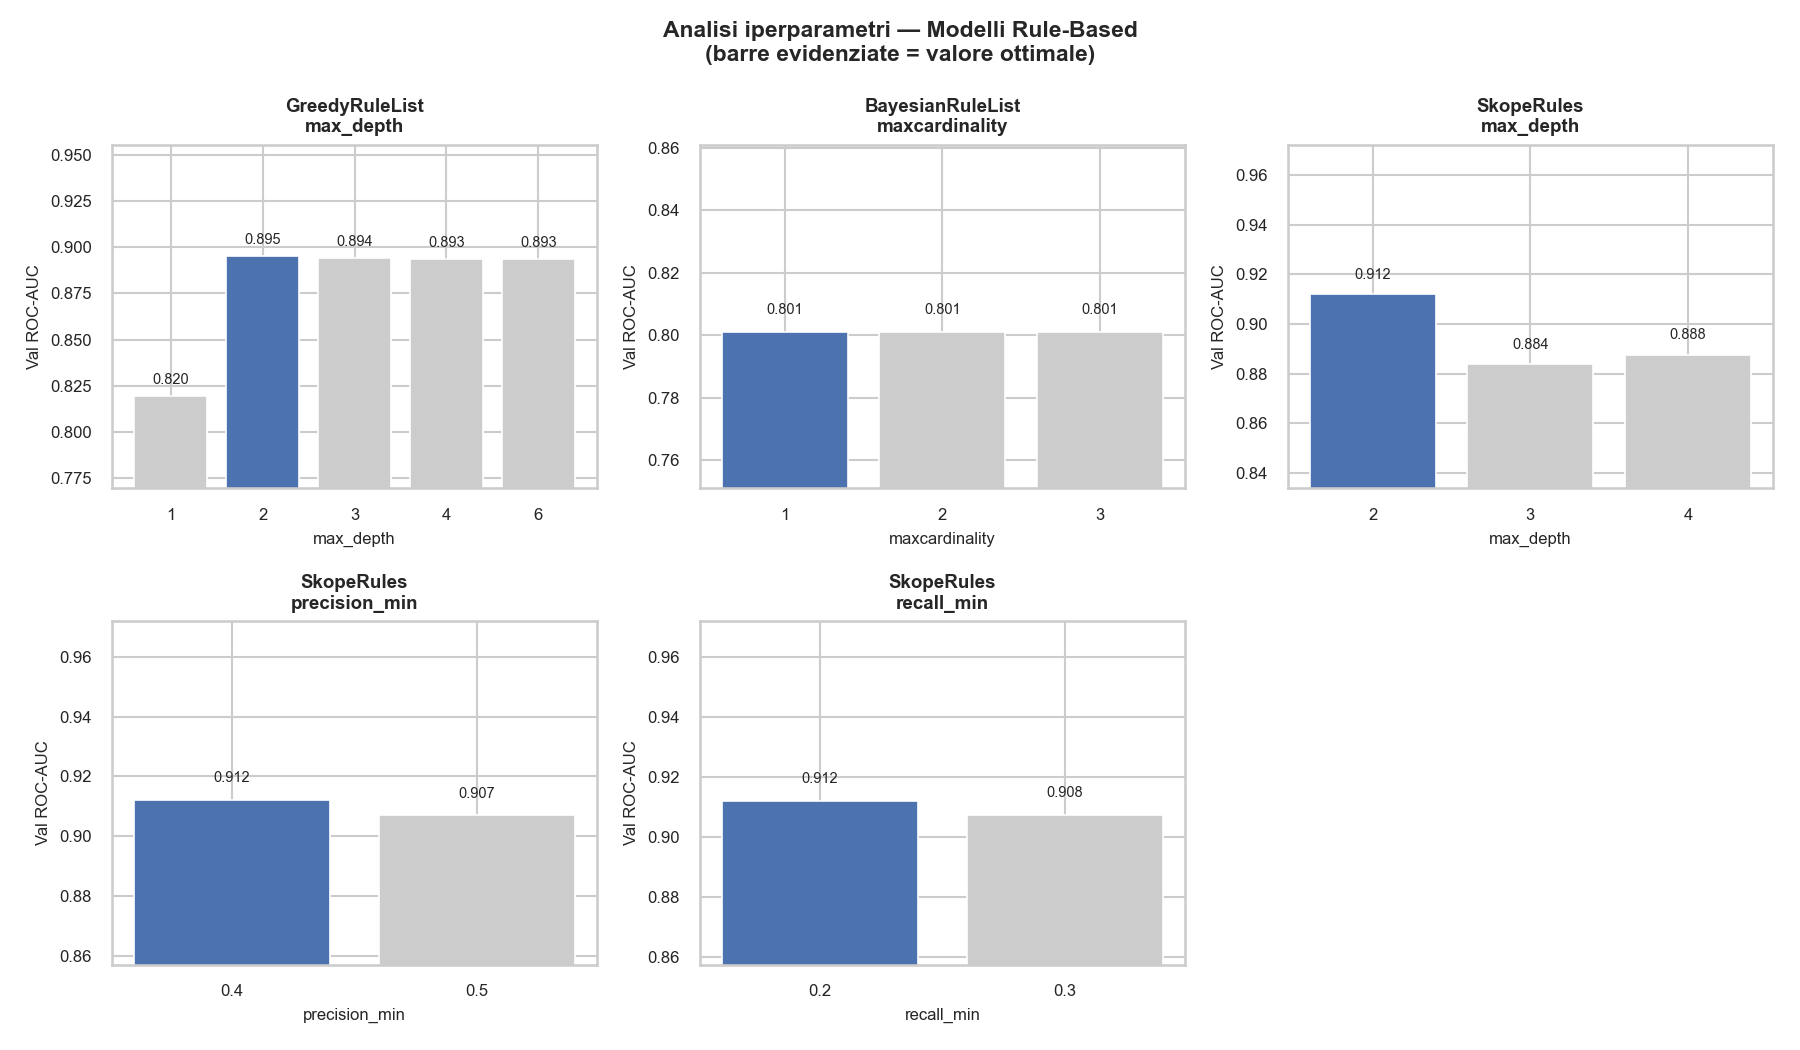
\includegraphics[width=\textwidth]{figures/hyperparam_rule_based.png}
\end{figure}

\clearpage
\textbf{Modelli ensemble.}
Tutti e tre i modelli mostrano scarsa sensibilità al numero di stimatori nell'intervallo
[100, 200]: la performance è già stabile a 100. Per Random Forest \texttt{max\_depth=None}
(alberi completi) domina; \texttt{min\_samples\_leaf=5} riduce la varianza su dataset piccoli.
Gradient Boosting e XGBoost preferiscono alberi poco profondi (max\_depth=3--4), coerente con
la dimensione ridotta del dataset.

\medskip
\begin{figure}[H]
  \centering
  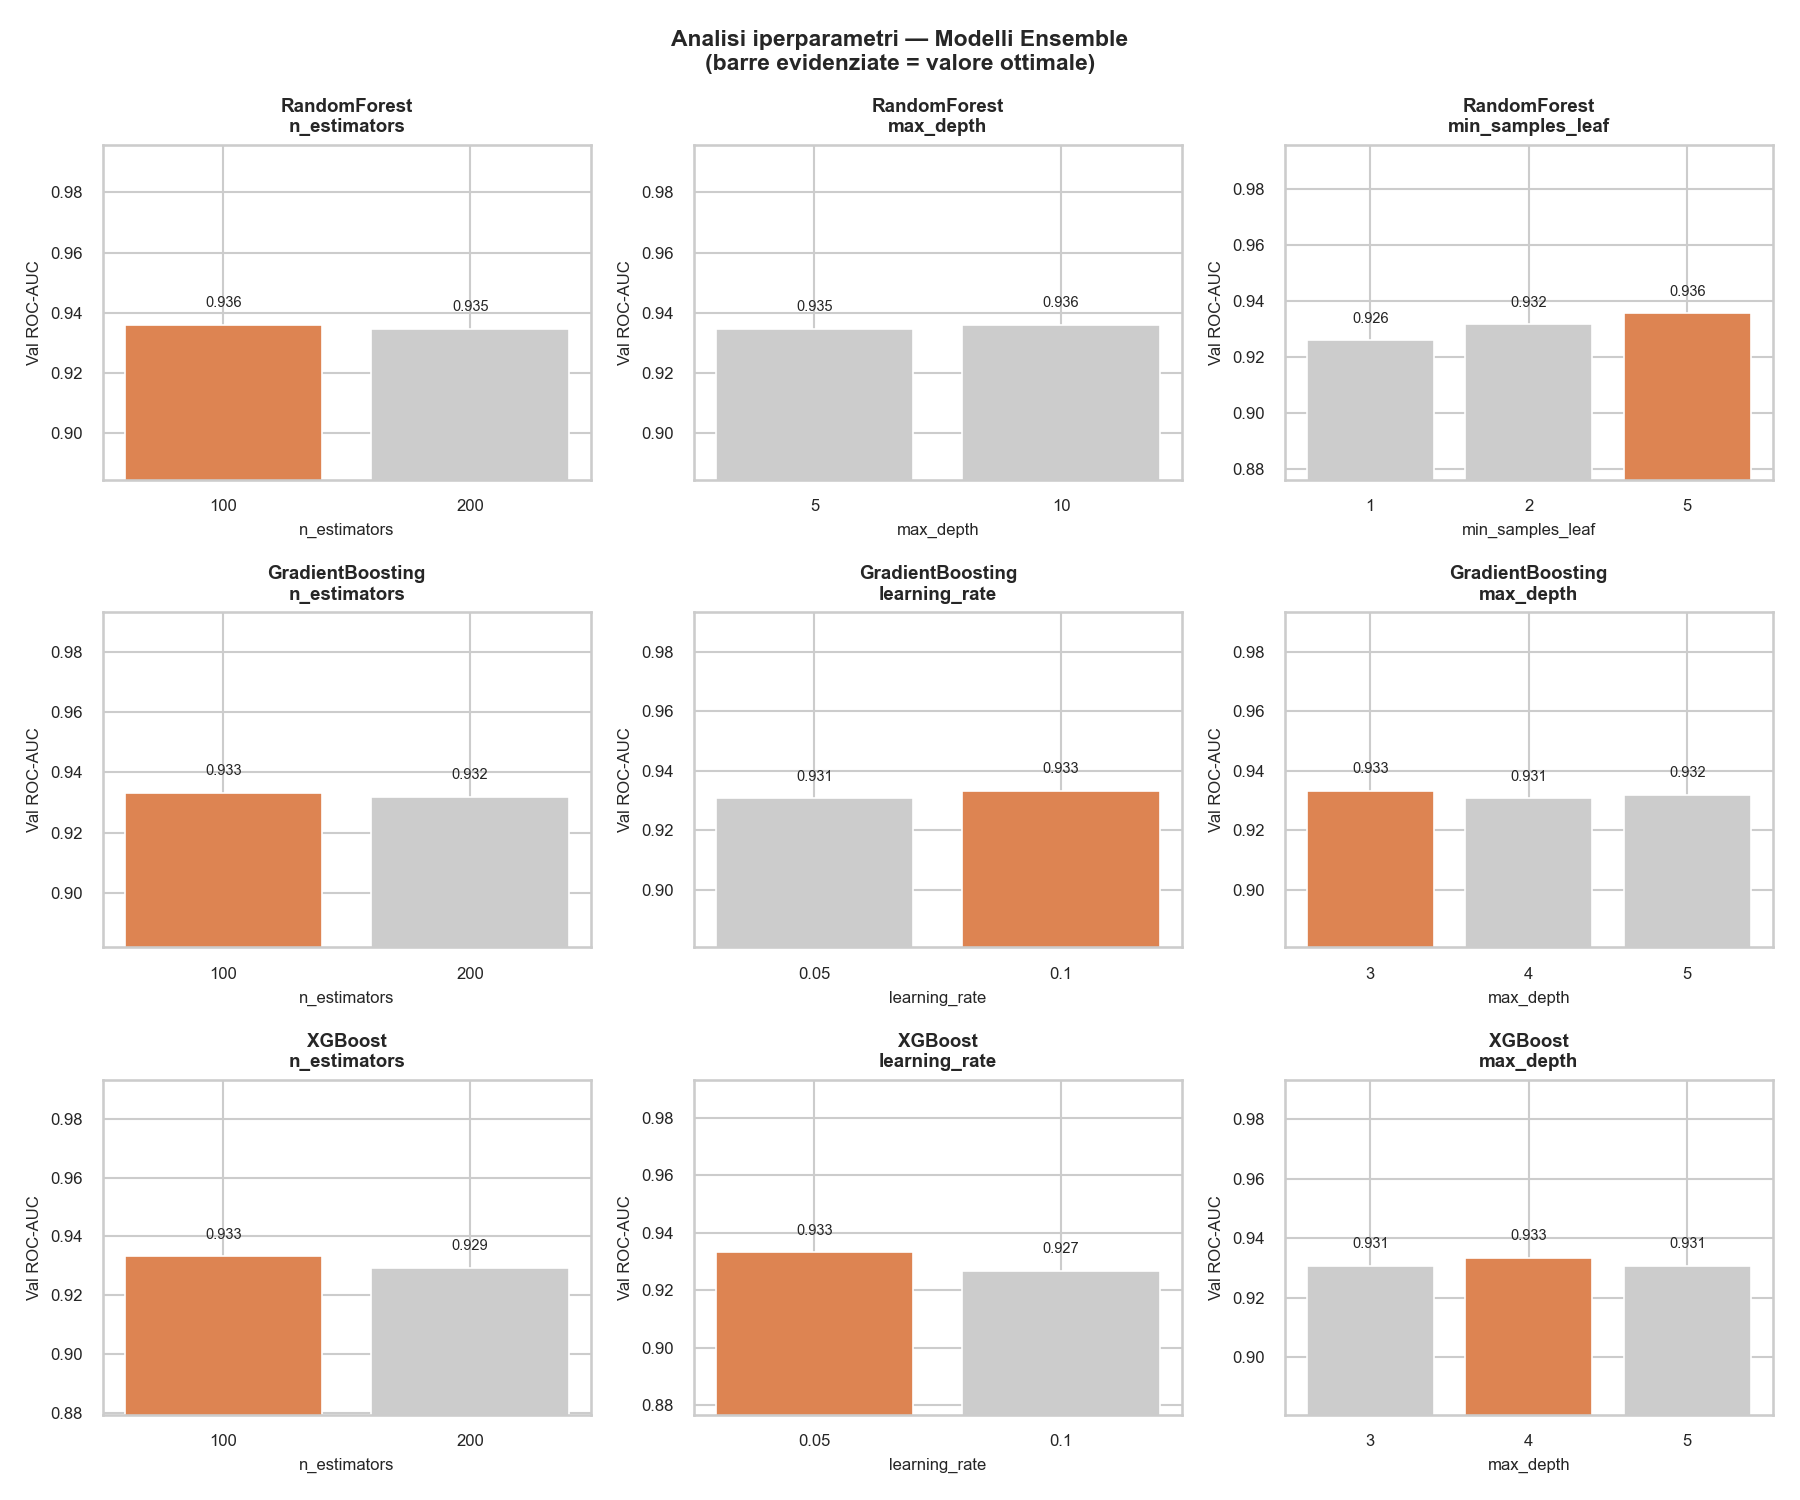
\includegraphics[width=\textwidth]{figures/hyperparam_ensemble.png}
\end{figure}


\section{Risultati}

\subsection{Metriche Comparative}

\begin{center}
{\small\begin{tabular}{>{\raggedright\arraybackslash}p{0.2164\linewidth}>{\raggedright\arraybackslash}p{0.1263\linewidth}>{\raggedright\arraybackslash}p{0.0902\linewidth}>{\raggedright\arraybackslash}p{0.0902\linewidth}>{\raggedright\arraybackslash}p{0.0902\linewidth}>{\raggedright\arraybackslash}p{0.0902\linewidth}>{\raggedright\arraybackslash}p{0.1082\linewidth}}
\toprule
\cellcolor{tblhdr}\color{white}\bfseries Modello & \cellcolor{tblhdr}\color{white}\bfseries Tipo & \cellcolor{tblhdr}\color{white}\bfseries Accuracy & \cellcolor{tblhdr}\color{white}\bfseries Precision & \cellcolor{tblhdr}\color{white}\bfseries Recall & \cellcolor{tblhdr}\color{white}\bfseries F1 & \cellcolor{tblhdr}\color{white}\bfseries ROC-AUC \\
\midrule
SkopeRules & Rule-based & 0.7000 & 1.0000 & 0.0526 & 0.1000 & 0.8960 \\
\rowcolor{ltrow}RandomForest & Ensemble & 0.8667 & 0.9231 & 0.6316 & 0.7500 & 0.8960 \\
XGBoost & Ensemble & 0.8667 & 0.8667 & 0.6842 & 0.7647 & 0.8434 \\
\rowcolor{ltrow}RuleFit & Rule-based & 0.8000 & 0.7692 & 0.5263 & 0.6250 & 0.8370 \\
GradientBoosting & Ensemble & 0.7500 & 0.6429 & 0.4737 & 0.5455 & 0.8344 \\
\rowcolor{ltrow}GreedyRuleList & Rule-based & 0.8333 & 0.9091 & 0.5263 & 0.6667 & 0.8331 \\
FIGS & Rule-based & 0.8000 & 0.7692 & 0.5263 & 0.6250 & 0.7677 \\
\rowcolor{ltrow}BayesianRuleList & Rule-based & 0.8000 & 0.7692 & 0.5263 & 0.6250 & 0.7651 \\
RIPPER & Rule-based & 0.7333 & 0.7143 & 0.2632 & 0.3846 & 0.6123 \\
\bottomrule
\end{tabular}}}
\end{center}

\medskip
\begin{figure}[H]
  \centering
  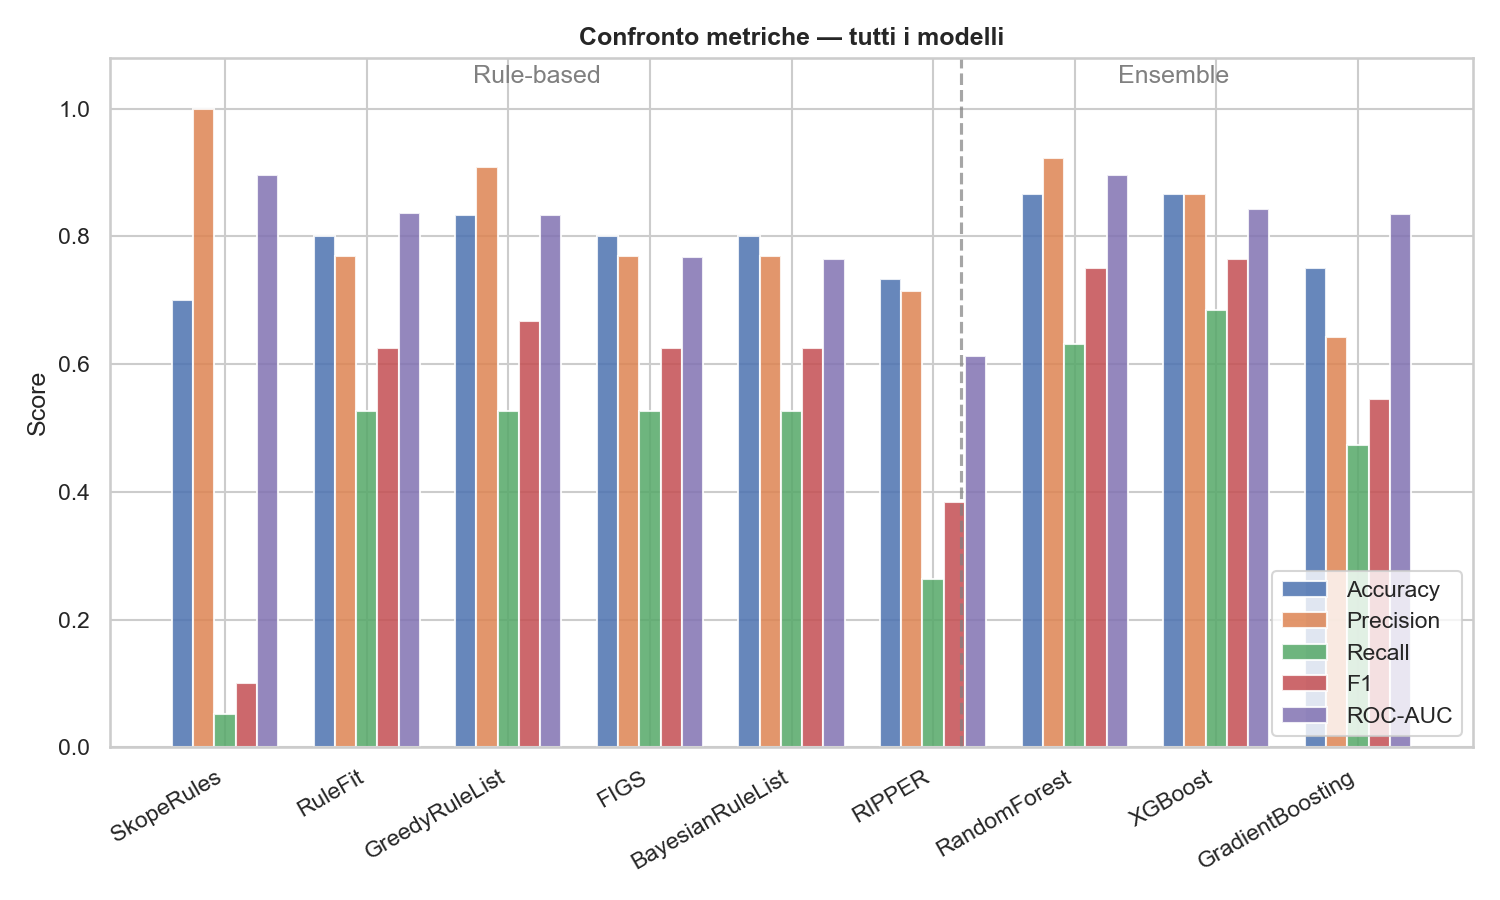
\includegraphics[width=\textwidth]{figures/metrics_comparison.png}
\end{figure}

Accuracy e F1 riassumono la qualità complessiva, ma su classi sbilanciate possono essere
fuorvianti. Precision misura quante predizioni ``deceduto'' sono corrette; Recall quante
morti reali vengono identificate --- in clinica un Recall basso è più pericoloso di una
Precision bassa. ROC-AUC è la metrica più robusta: misura la capacità di separare le classi
indipendentemente dalla soglia.
GreedyRuleList raggiunge buon F1 e Accuracy con regole a condizione singola.
SkopeRules ottiene Precision=1.0 con Recall molto basso: identifica pochi deceduti ma senza
mai sbagliare. RIPPER produce regole congiuntive (AND) ma ha il ROC-AUC più basso tra tutti i
modelli, dimostrando che la complessità strutturale non implica migliore capacità discriminativa.

\clearpage
\subsection{Curve ROC}

\begin{figure}[H]
  \centering
  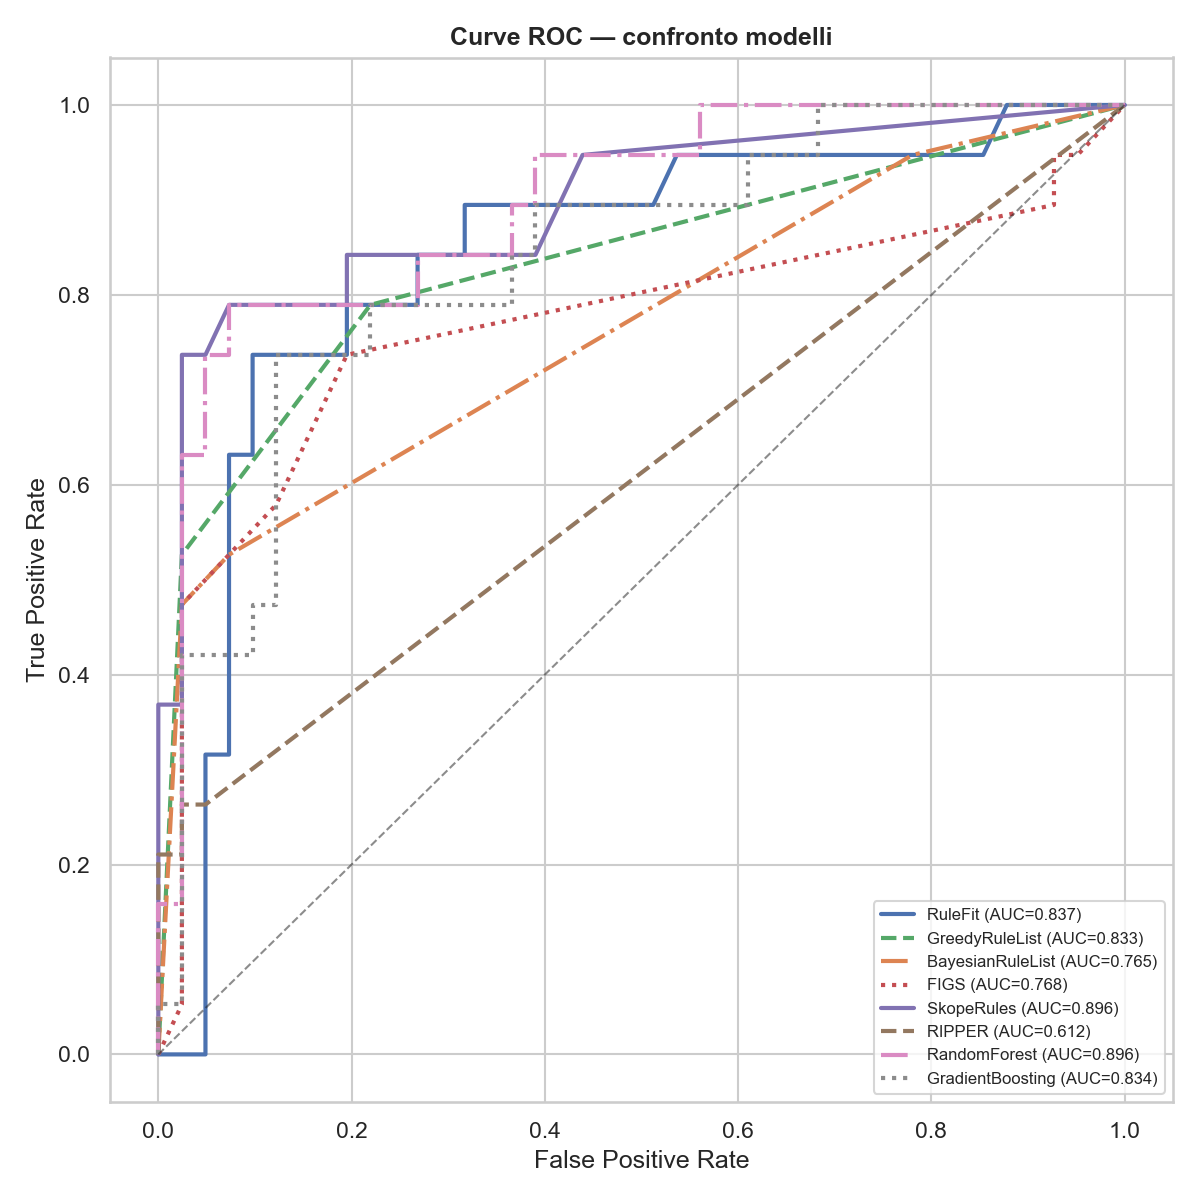
\includegraphics[width=\textwidth]{figures/roc_curves.png}
\end{figure}

La curva ROC traccia il TPR (Recall) contro il FPR al variare della soglia; l'AUC riassume
la performance in un unico numero indipendente dalla soglia (0.50\,=\,casuale, 1.0\,=\,perfetto).
Random Forest raggiunge l'AUC più alto tra tutti i modelli. SkopeRules e GreedyRuleList mostrano
risultati notevoli per modelli intrinsecamente interpretabili. RIPPER ha l'AUC più basso: nonostante
F1 e Accuracy competitivi, il ranking probabilistico è meno calibrato.

\clearpage
\subsection{Matrici di Confusione}

\begin{figure}[H]
  \centering
  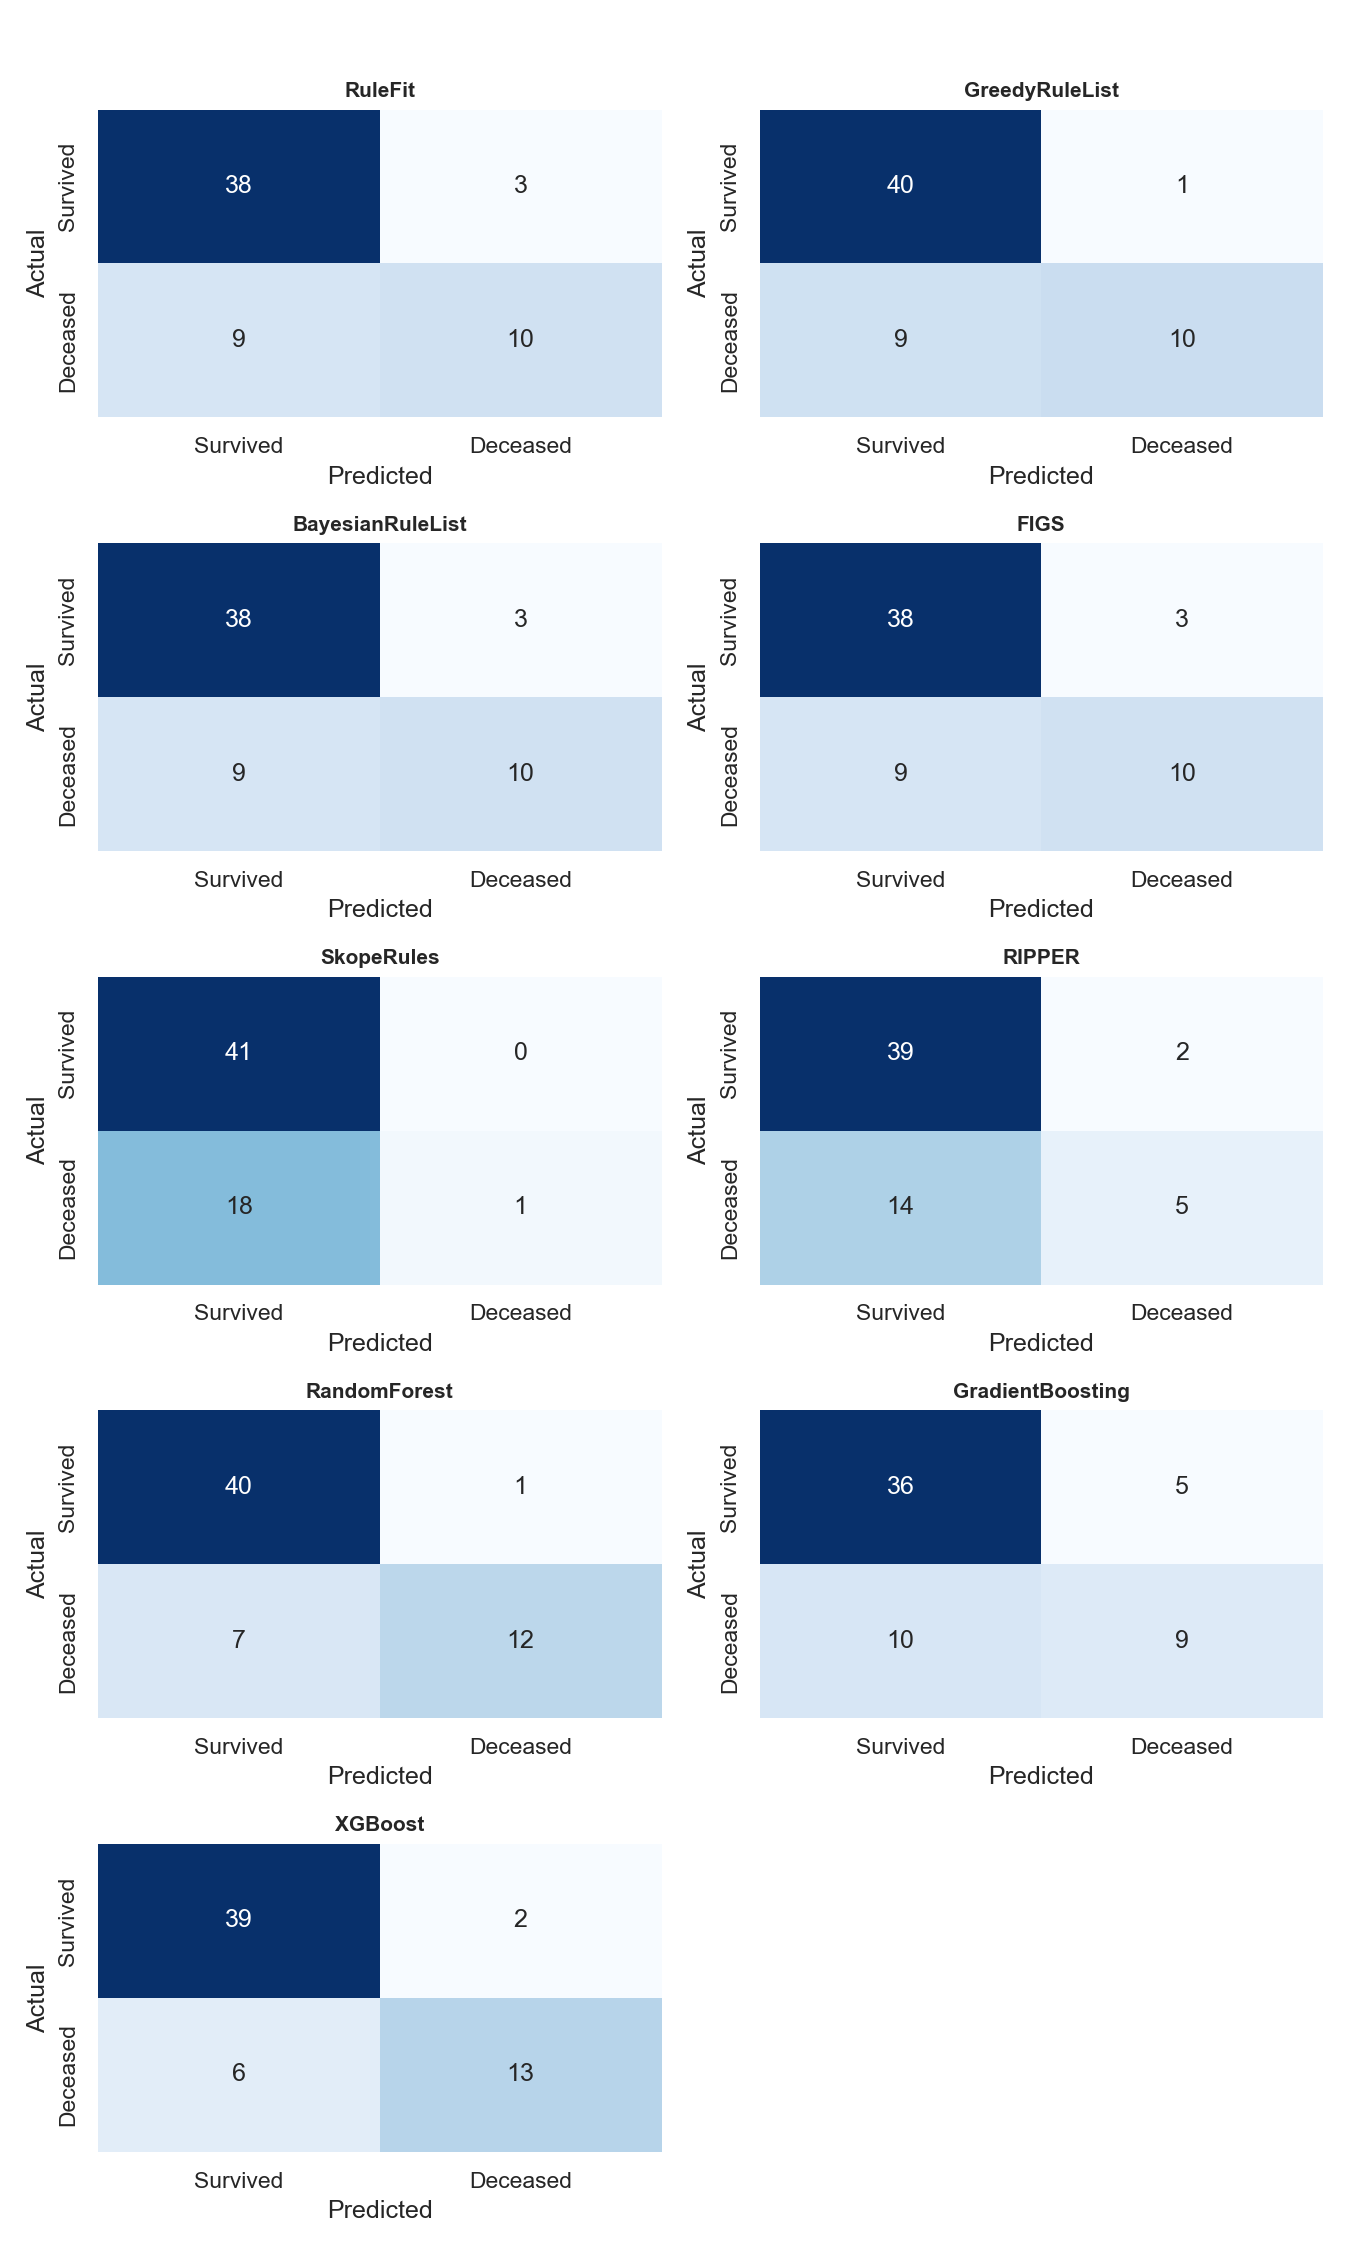
\includegraphics[width=\textwidth]{figures/confusion_matrices.png}
\end{figure}

Ogni cella indica: riga = classe reale, colonna = classe predetta. La diagonale raccoglie le
predizioni corrette; gli elementi fuori diagonale sono gli errori. In clinica i due tipi di
errore hanno costo asimmetrico: un falso negativo (morte non rilevata) è più grave di un falso
positivo (falso allarme). BayesianRuleList massimizza il Recall sui deceduti --- pochi falsi
negativi --- a scapito di più falsi positivi. Gli ensemble bilanciano meglio i due errori.
SkopeRules ha Precision=1.0 ma Recall molto basso: identifica pochi deceduti, senza mai
produrre falsi positivi.

\clearpage
\subsection{Regole Complete: tutti i modelli interpretabili}

\textbf{GreedyRuleList.}
Lista IF/THEN sequenziale: la prima regola soddisfatta determina la classe, che non è
necessariamente Decesso --- ogni regola predice la classe di maggioranza del proprio segmento
($>$50\% deceduti $\Rightarrow$ Decesso). GRL è strutturalmente limitato a una condizione per
regola; il parametro \texttt{max\_depth} controlla la lunghezza della lista.

\medskip
\begin{center}
{\small\begin{tabular}{>{\raggedright\arraybackslash}p{0.3278\linewidth}>{\raggedright\arraybackslash}p{0.1035\linewidth}>{\raggedright\arraybackslash}p{0.1035\linewidth}>{\raggedright\arraybackslash}p{0.1898\linewidth}>{\raggedright\arraybackslash}p{0.1380\linewidth}}
\toprule
\cellcolor{tblhdr}\color{white}\bfseries Condizione & \cellcolor{tblhdr}\color{white}\bfseries Precisione & \cellcolor{tblhdr}\color{white}\bfseries Recall & \cellcolor{tblhdr}\color{white}\bfseries Predizione & \cellcolor{tblhdr}\color{white}\bfseries Campioni \\
\midrule
time <= 73.500 & 0.830 & 0.672 & Decesso & 47 \\
\rowcolor{ltrow}serum\_creatinine > 1.450 & 0.500 & 0.091 & Sopravvissuto & 22 \\
DEFAULT & 0.927 & 0.843 & Sopravvissuto & 110 \\
\bottomrule
\end{tabular}}}
\end{center}

\medskip
\textbf{BayesianRuleList.}
Lista IF/ELSE con MCMC su feature discretizzate. Ogni antecedente ha al massimo
\texttt{maxcardinality} condizioni congiuntive; il valore ottimale (1) è stato
scelto sul validation set. P(decesso) è la probabilità posteriore con IC al 95\%.

\medskip
\begin{center}
{\small\begin{tabular}{>{\raggedright\arraybackslash}p{0.5299\linewidth}>{\raggedright\arraybackslash}p{0.1827\linewidth}>{\raggedright\arraybackslash}p{0.2010\linewidth}}
\toprule
\cellcolor{tblhdr}\color{white}\bfseries Condizione & \cellcolor{tblhdr}\color{white}\bfseries P(decesso) & \cellcolor{tblhdr}\color{white}\bfseries IC 95\textbackslash{}\% \\
\midrule
serum\_creatinine $\in$ (0.50, 0.90] & 6.1\% & 0.8\%--16.2\% \\
\rowcolor{ltrow}time $\in$ (6.00, 71.50] & 84.4\% & 72.6\%--93.4\% \\
ejection\_fraction $\in$ (15.00, 30.00] & 51.9\% & 33.4\%--70.1\% \\
\rowcolor{ltrow}DEFAULT (nessuna regola attivata) & 9.8\% & 4.4\%--17.0\% \\
\bottomrule
\end{tabular}}}
\end{center}

\medskip
\textbf{RIPPER.}
Ogni regola ha un antecedente con più condizioni AND (tutte devono essere verificate
simultaneamente). Se tutte le condizioni di una regola sono soddisfatte $\Rightarrow$ Decesso;
nessuna regola soddisfatta $\Rightarrow$ Sopravvissuto (DEFAULT).

\medskip
\begin{center}
{\small\begin{tabular}{>{\raggedright\arraybackslash}p{0.3278\linewidth}>{\raggedright\arraybackslash}p{0.1553\linewidth}>{\raggedright\arraybackslash}p{0.1035\linewidth}>{\raggedright\arraybackslash}p{0.1035\linewidth}>{\raggedright\arraybackslash}p{0.1725\linewidth}}
\toprule
\cellcolor{tblhdr}\color{white}\bfseries Regola & \cellcolor{tblhdr}\color{white}\bfseries Predizione & \cellcolor{tblhdr}\color{white}\bfseries Precisione & \cellcolor{tblhdr}\color{white}\bfseries Recall & \cellcolor{tblhdr}\color{white}\bfseries Campioni \\
\midrule
time <= 28.8 & Decesso & 1.000 & 0.310 & 18 \\
\rowcolor{ltrow}ejection\_fraction <= 25.0 AND high\_blood\_pressure = 1 & Decesso & 0.769 & 0.172 & 13 \\
ejection\_fraction <= 25.0 AND platelets $\in$ (197200.0, 220400.0] & Decesso & 1.000 & 0.069 & 4 \\
\rowcolor{ltrow}time $\in$ (28.8, 57.4] AND sex = 0 & Decesso & 0.875 & 0.121 & 8 \\
DEFAULT & Sopravvissuto & 0.860 & 0.967 & 136 \\
\bottomrule
\end{tabular}}}
\end{center}

\clearpage
\textbf{RuleFit --- regole con coefficiente positivo (pro Decesso).}
Ogni regola è un percorso estratto da un ensemble di alberi; il coefficiente Lasso indica
il peso nella predizione finale. Valori più alti indicano maggiore contributo al rischio di
decesso. Le regole possono combinare più feature (AND implicito sul percorso).

\medskip
\begin{center}
{\small\begin{tabular}{>{\raggedright\arraybackslash}p{0.7700\linewidth}>{\raggedright\arraybackslash}p{0.1690\linewidth}}
\toprule
\cellcolor{tblhdr}\color{white}\bfseries Regola & \cellcolor{tblhdr}\color{white}\bfseries Coefficiente \\
\midrule
time <= 0.67896 and time > 0.23773 & 3.147 \\
\rowcolor{ltrow}time <= -0.62527 and serum\_creatinine > -0.44392 & 1.342 \\
time > -0.69016 and creatinine\_phosphokinase <= -0.01926 and creatinine\_phosphokinase > -0.33791 and serum\_creatinine > -0.14962 & 1.263 \\
\rowcolor{ltrow}time <= 0.67896 & 1.130 \\
time > -0.67718 and creatinine\_phosphokinase > 0.25316 and ejection\_fraction <= -0.41598 and serum\_creatinine > -0.50523 & 1.006 \\
\rowcolor{ltrow}time > -0.68367 and creatinine\_phosphokinase <= -0.01926 and creatinine\_phosphokinase > -0.49123 and serum\_creatinine > 0.16921 & 0.877 \\
time <= -0.67718 and serum\_creatinine <= 0.35315 and serum\_creatinine > -0.56654 & 0.704 \\
\rowcolor{ltrow}time <= -1.02108 and creatinine\_phosphokinase <= 1.22865 & 0.622 \\
\bottomrule
\end{tabular}}}
\end{center}

\medskip
\textbf{SkopeRules.}
Regole ad alta precisione estratte tramite sub-campionamenti di ensemble di alberi, poi
de-duplicate. La profondità degli alberi base (\texttt{max\_depth} ottimizzato sul validation
set) controlla il numero di condizioni per regola. Ogni regola è corredata da Precisione e
Recall sul training set.

\medskip
{\small
\begin{longtable}{>{\raggedright\arraybackslash}p{0.5847\linewidth}>{\raggedright\arraybackslash}p{0.1644\linewidth}>{\raggedright\arraybackslash}p{0.1644\linewidth}}
\toprule
\cellcolor{tblhdr}\color{white}\bfseries Regola & \cellcolor{tblhdr}\color{white}\bfseries Precisione & \cellcolor{tblhdr}\color{white}\bfseries Recall \\
\midrule
\endfirsthead
\toprule
\cellcolor{tblhdr}\color{white}\bfseries Regola & \cellcolor{tblhdr}\color{white}\bfseries Precisione & \cellcolor{tblhdr}\color{white}\bfseries Recall \\
\midrule
\endhead
\midrule
\endlastfoot
time <= 78.5 and serum\_creatinine > 0.85 & 0.837 & 0.707 \\
time <= 78.5 and serum\_creatinine > 0.75 & 0.820 & 0.707 \\
time <= 73.5 and serum\_creatinine > 0.75 & 0.848 & 0.672 \\
time <= 67.5 and serum\_creatinine > 0.75 & 0.881 & 0.638 \\
time <= 73.5 and serum\_creatinine > 0.85 & 0.867 & 0.672 \\
time <= 78.5 and ejection\_fraction > 27.5 & 0.703 & 0.448 \\
time <= 73.5 and serum\_creatinine > 0.95 & 0.878 & 0.621 \\
time <= 67.5 and creatinine\_phosphokinase <= 142.0 & 0.800 & 0.207 \\
time <= 69.0 and high\_blood\_pressure <= 0.5 & 0.727 & 0.276 \\
time <= 67.5 & 0.860 & 0.638 \\
ejection\_fraction <= 32.5 and serum\_creatinine <= 1.815 & 0.521 & 0.431 \\
time <= 66.5 and serum\_creatinine > 0.75 & 0.878 & 0.621 \\
age <= 61.0 and time <= 78.0 & 0.720 & 0.310 \\
ejection\_fraction > 22.5 and serum\_creatinine > 1.45 & 0.606 & 0.345 \\
time <= 67.5 and time > 28.5 & 0.760 & 0.328 \\
time <= 52.0 & 0.909 & 0.517 \\
time <= 78.5 and time > 28.5 & 0.676 & 0.397 \\
serum\_creatinine > 1.45 and serum\_sodium > 130.5 & 0.706 & 0.414 \\
time <= 73.5 and high\_blood\_pressure <= 0.5 & 0.720 & 0.310 \\
creatinine\_phosphokinase > 89.5 and serum\_creatinine > 1.45 & 0.759 & 0.379 \\
time > 73.5 and ejection\_fraction <= 32.5 & 0.366 & 0.259 \\
time <= 73.5 and high\_blood\_pressure > 0.5 & 0.955 & 0.362 \\
ejection\_fraction > 27.5 and serum\_creatinine > 1.45 & 0.667 & 0.276 \\
time <= 55.0 & 0.861 & 0.534 \\
time <= 73.5 and time > 28.5 & 0.724 & 0.362 \\
time <= 67.5 and creatinine\_phosphokinase > 142.0 & 0.893 & 0.431 \\
time <= 73.5 and serum\_sodium <= 136.5 & 0.960 & 0.414 \\
time <= 28.5 & 1.000 & 0.310 \\
time <= 73.5 and serum\_sodium > 136.5 & 0.682 & 0.259 \\
time <= 73.5 and platelets > 124500.0 & 0.844 & 0.655 \\
ejection\_fraction <= 27.5 and serum\_creatinine > 0.85 & 0.676 & 0.431 \\
creatinine\_phosphokinase > 71.0 and ejection\_fraction <= 27.5 & 0.676 & 0.431 \\
time <= 73.5 and time > 28.0 & 0.724 & 0.362 \\
ejection\_fraction <= 27.5 and serum\_creatinine <= 1.45 & 0.615 & 0.276 \\
creatinine\_phosphokinase > 75.5 and serum\_creatinine > 1.45 & 0.767 & 0.397 \\
time <= 67.5 and time > 28.0 & 0.760 & 0.328 \\
time > 52.0 and serum\_creatinine <= 1.45 & 0.124 & 0.259 \\
time > 67.5 and ejection\_fraction <= 27.5 & 0.464 & 0.224 \\
time <= 28.0 & 1.000 & 0.310 \\
time <= 66.5 and time > 28.5 & 0.750 & 0.310 \\
time > 66.5 and ejection\_fraction <= 32.5 & 0.395 & 0.293 \\
ejection\_fraction > 27.5 and serum\_creatinine > 1.815 & 0.786 & 0.190 \\
time <= 78.5 and time > 55.0 & 0.625 & 0.172 \\
time <= 78.0 and time > 28.5 & 0.676 & 0.397 \\
ejection\_fraction <= 32.5 and serum\_creatinine > 0.95 & 0.646 & 0.534 \\
time > 73.5 and serum\_creatinine > 1.55 & 0.500 & 0.172 \\
creatinine\_phosphokinase > 59.5 and serum\_creatinine > 1.45 & 0.727 & 0.414 \\
ejection\_fraction <= 27.5 and platelets <= 195000.0 & 0.375 & 0.052 \\
time <= 69.0 and high\_blood\_pressure > 0.5 & 0.955 & 0.362 \\
time > 73.5 and serum\_creatinine > 1.45 & 0.500 & 0.190 \\
time <= 67.5 and serum\_sodium > 136.5 & 0.750 & 0.259 \\
time <= 67.5 and serum\_sodium <= 136.5 & 0.957 & 0.379 \\
ejection\_fraction <= 22.5 & 0.917 & 0.190 \\
creatinine\_phosphokinase > 69.0 and serum\_creatinine > 1.45 & 0.742 & 0.397 \\
ejection\_fraction <= 27.5 and platelets > 195000.0 & 0.688 & 0.379 \\
ejection\_fraction <= 27.5 and ejection\_fraction > 22.5 & 0.500 & 0.241 \\
time > 73.5 and ejection\_fraction <= 27.5 & 0.444 & 0.207 \\
ejection\_fraction > 27.5 and serum\_sodium <= 134.5 & 0.412 & 0.241 \\
platelets <= 319000.0 and serum\_creatinine > 1.45 & 0.594 & 0.328 \\
time > 78.5 and ejection\_fraction <= 22.5 & 0.800 & 0.069 \\
time > 66.5 and ejection\_fraction <= 27.5 & 0.483 & 0.241 \\
ejection\_fraction > 27.5 and serum\_creatinine > 1.85 & 0.750 & 0.155 \\
time > 52.0 and serum\_creatinine > 1.45 & 0.520 & 0.224 \\
age > 61.0 and time <= 78.0 & 0.852 & 0.397 \\
\end{longtable}
}

\clearpage
\textbf{FIGS --- Fast Interpretable Greedy-Tree Sums.}
FIGS è una somma di alberi: ogni albero assegna al campione un valore numerico e se la somma
supera 0.5 la predizione è Decesso. Di seguito la struttura completa degli alberi appresi:

\medskip
\begin{small}
\begin{verbatim}
> ------------------------------
> FIGS-Fast Interpretable Greedy-Tree Sums:
> 	Predictions are made by summing the "Val" reached by traversing each tree.
> 	For classifiers, a softmax function is then applied to the sum.
> ------------------------------
time <= 73.500 (Tree #0 root)
	time <= 52.000 (split)
		Val: 0.077 0.923 (leaf)
		serum_sodium <= 137.000 (split)
			Val: 0.163 0.837 (leaf)
			ejection_fraction <= 30.000 (split)
				Val: 0.258 0.742 (leaf)
				Val: 0.926 0.074 (leaf)
	serum_creatinine <= 1.450 (split)
		Val: 0.898 0.102 (leaf)
		creatinine_phosphokinase <= 69.000 (split)
			Val: 1.059 -0.059 (leaf)
			time <= 104.000 (split)
				Val: 0.125 0.875 (leaf)
				serum_creatinine <= 1.965 (split)
					Val: 0.492 0.508 (leaf)
					Val: 1.258 -0.258 (leaf)

	+
ejection_fraction <= 27.500 (Tree #1 root)
	time <= 148.000 (split)
		Val: -0.104 0.104 (leaf)
		Val: -0.36 0.36 (leaf)
	Val: 0.074 -0.074 (leaf)
\end{verbatim}
\end{small}

\clearpage
\subsection{Cross-Validation 10-fold}

\begin{figure}[H]
  \centering
  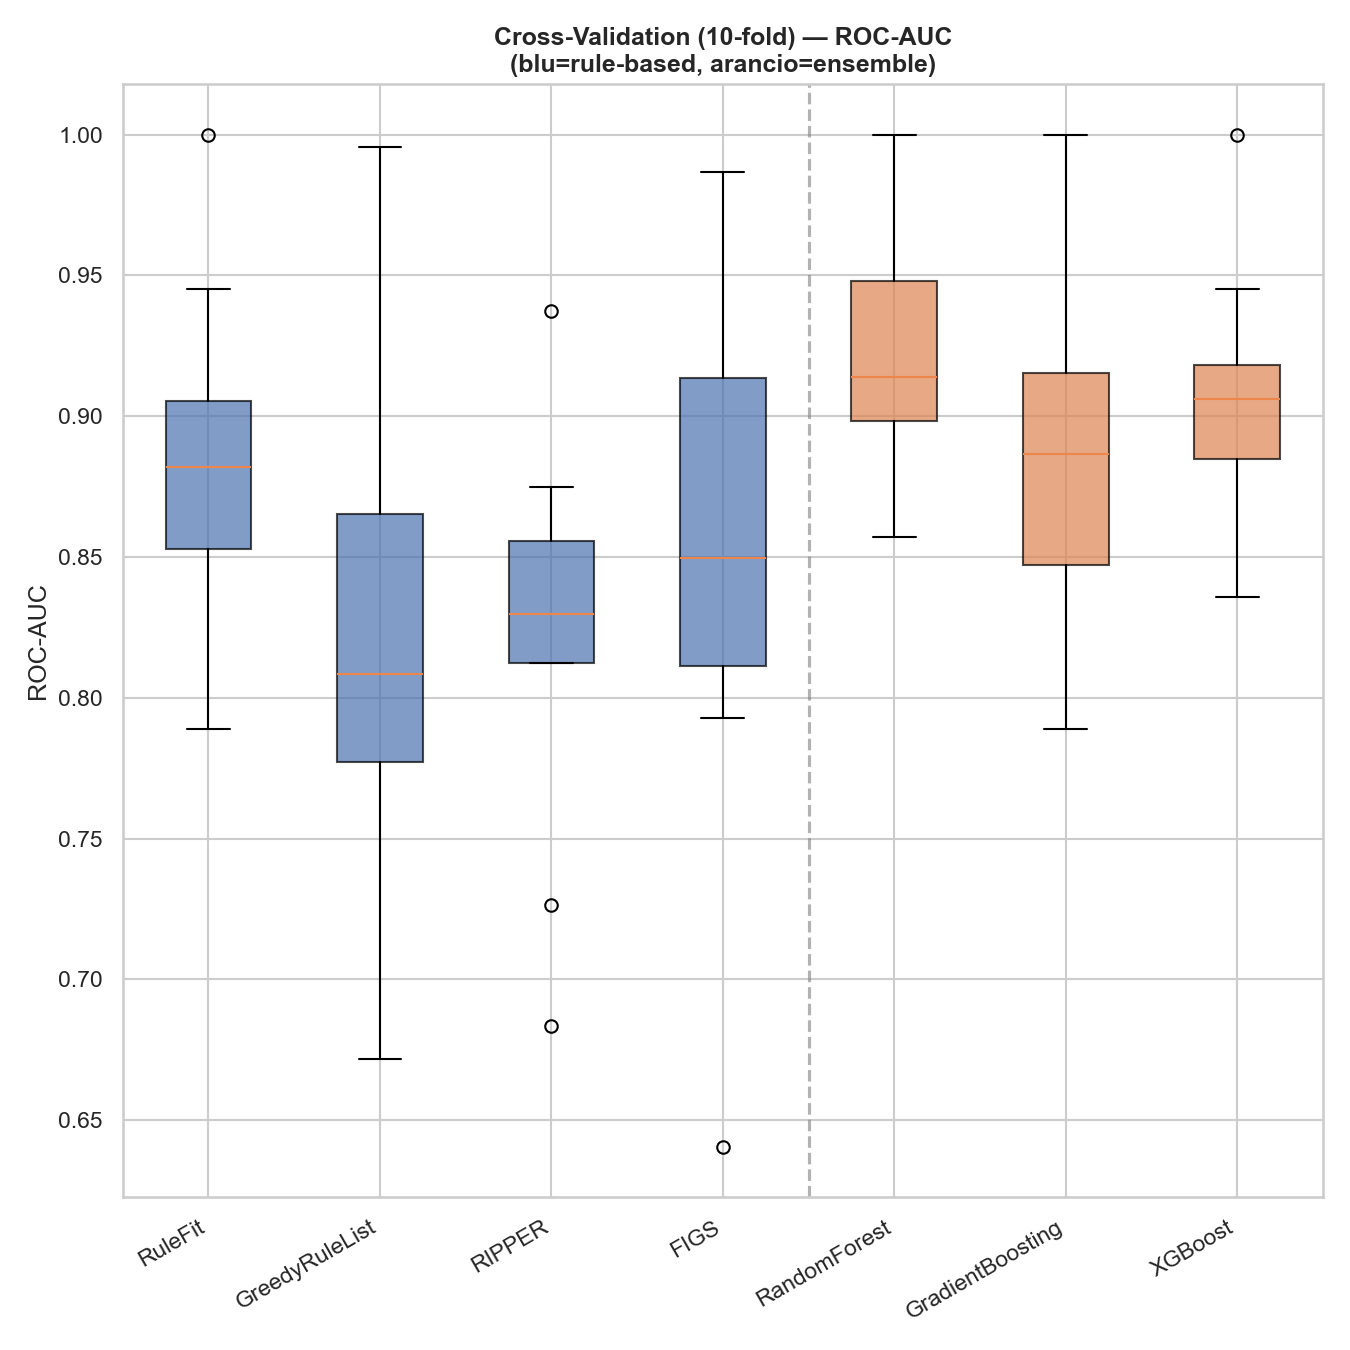
\includegraphics[width=\textwidth]{figures/cross_validation.png}
\end{figure}

Il boxplot mostra la distribuzione del ROC-AUC su 10 fold stratificati del set trainval
($\approx$240 campioni): mediana, IQR (bordi del box) e range (baffi). La stratificazione
garantisce che ogni fold mantenga la stessa proporzione di deceduti ($\sim$32\%). I modelli
usano gli iperparametri ottimizzati sul validation set. Random Forest ha la mediana più alta e
IQR contenuto: performance stabile e consistente. RuleFit è il miglior rule-based in CV.
FIGS mostra alta varianza --- instabile su dataset piccoli. GreedyRuleList usa un custom scorer
che aggira un'incompatibilità con l'API sklearn.

\clearpage
\subsection{RF e GRL senza feature \texttt{time}}

\textbf{Motivazione.}
La feature \texttt{time} (durata del follow-up) è la più predittiva del dataset. In contesti
reali di triage questa informazione non è sempre disponibile al momento della prima valutazione.
Questo esperimento valuta RF e GRL privandoli di \texttt{time}, forzandoli ad appoggiarsi ai
segnali biochimici e demografici rimanenti. RF e GRL vengono ri-tunati sul proprio validation
set (senza \texttt{time}) per garantire un confronto equo.

\medskip
\begin{center}
{\small\begin{tabular}{>{\raggedright\arraybackslash}p{0.3552\linewidth}>{\raggedright\arraybackslash}p{0.1776\linewidth}>{\raggedright\arraybackslash}p{0.1776\linewidth}>{\raggedright\arraybackslash}p{0.1776\linewidth}}
\toprule
\cellcolor{tblhdr}\color{white}\bfseries Modello & \cellcolor{tblhdr}\color{white}\bfseries Accuracy & \cellcolor{tblhdr}\color{white}\bfseries F1 & \cellcolor{tblhdr}\color{white}\bfseries ROC-AUC \\
\midrule
RandomForest & 0.8667 & 0.7500 & 0.8960 \\
\rowcolor{ltrow}RF\textbackslash{}\_no\textbackslash{}\_time & 0.7500 & 0.5161 & 0.7754 \\
GreedyRuleList & 0.8333 & 0.6667 & 0.8331 \\
\rowcolor{ltrow}GRL\textbackslash{}\_no\textbackslash{}\_time & 0.6833 & 0.5366 & 0.7003 \\
\bottomrule
\end{tabular}}}
\end{center}

\medskip
Rimuovendo \texttt{time}, il ROC-AUC scende di circa 0.10 per entrambi i modelli: un costo
atteso dato il peso dominante di \texttt{time}. Senza di essa i modelli si affidano a
\texttt{serum\_creatinine} ed \texttt{ejection\_fraction} --- feature biochimiche disponibili
alla prima valutazione, prima del follow-up --- e rimangono utilizzabili in contesti di triage.

\medskip
\textbf{Regole GRL senza \texttt{time}.}
Con la rimozione di \texttt{time}, GreedyRuleList apprende dai segnali biochimici:
\texttt{serum\_creatinine} ed \texttt{ejection\_fraction} diventano le feature dominanti.

\medskip
\begin{center}
{\small\begin{tabular}{>{\raggedright\arraybackslash}p{0.3278\linewidth}>{\raggedright\arraybackslash}p{0.1035\linewidth}>{\raggedright\arraybackslash}p{0.1035\linewidth}>{\raggedright\arraybackslash}p{0.1898\linewidth}>{\raggedright\arraybackslash}p{0.1380\linewidth}}
\toprule
\cellcolor{tblhdr}\color{white}\bfseries Condizione & \cellcolor{tblhdr}\color{white}\bfseries Precisione & \cellcolor{tblhdr}\color{white}\bfseries Recall & \cellcolor{tblhdr}\color{white}\bfseries Predizione & \cellcolor{tblhdr}\color{white}\bfseries Campioni \\
\midrule
serum\_creatinine > 1.450 & 0.658 & 0.431 & Decesso & 38 \\
\rowcolor{ltrow}ejection\_fraction <= 27.500 & 0.615 & 0.276 & Decesso & 26 \\
creatinine\_phosphokinase > 5211.000 & 1.000 & 0.034 & Decesso & 2 \\
\rowcolor{ltrow}age > 81.500 & 0.500 & 0.025 & Sopravvissuto & 6 \\
diabetes > 0.500 & 0.816 & 0.331 & Sopravvissuto & 49 \\
\rowcolor{ltrow}serum\_creatinine <= 0.650 & 0.667 & 0.017 & Sopravvissuto & 3 \\
DEFAULT & 0.964 & 0.438 & Sopravvissuto & 55 \\
\bottomrule
\end{tabular}}}
\end{center}

\clearpage
\subsection{Interpretabilità}

\textbf{Regole RuleFit --- coefficienti Lasso.}

\begin{figure}[H]
  \centering
  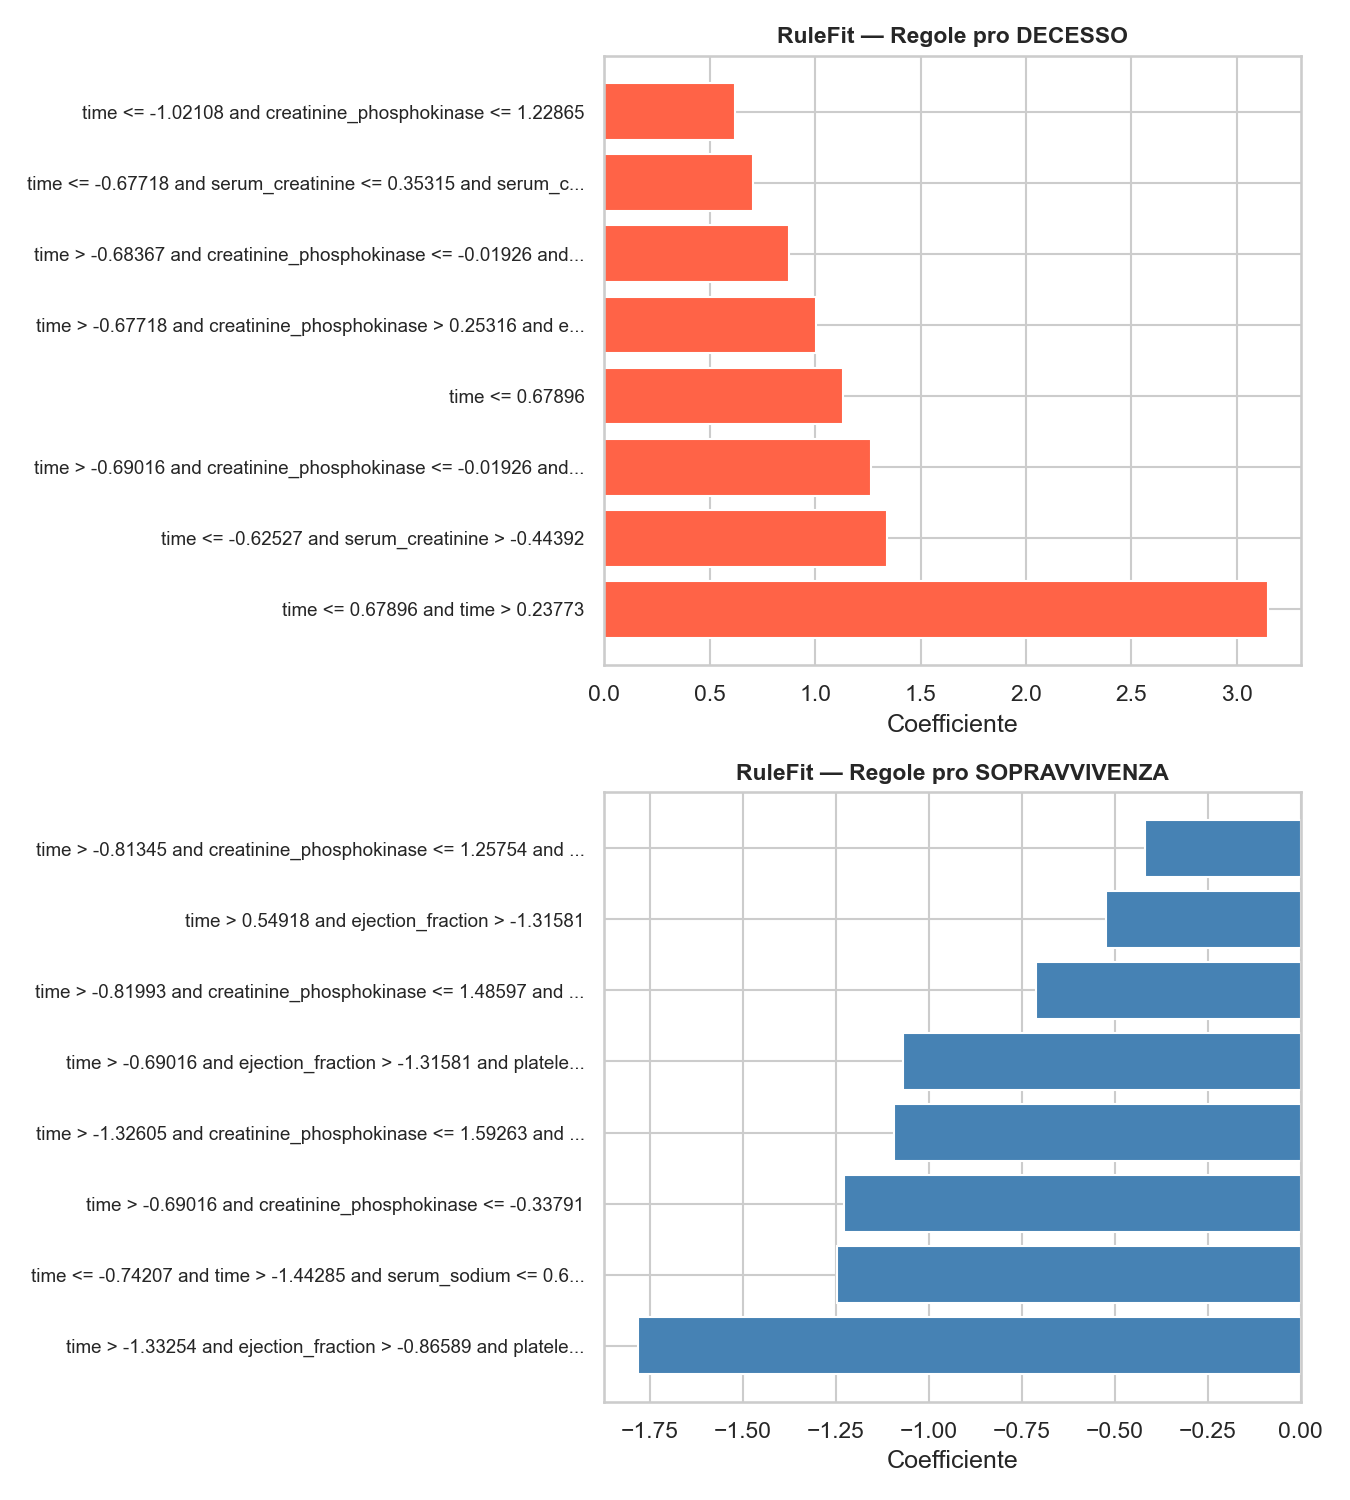
\includegraphics[width=\textwidth]{figures/rulefit_rules.png}
\end{figure}

Coefficienti Lasso delle regole estratte da RuleFit: positivo (barre rosse) $\Rightarrow$ la
regola aumenta il rischio di decesso; negativo (blu) $\Rightarrow$ lo riduce. Le regole
pro-decesso con peso più alto coinvolgono \texttt{time} basso e \texttt{serum\_creatinine}
alta. Le regole pro-sopravvivenza implicano \texttt{ejection\_fraction} più alta e follow-up
lungo. La penalizzazione Lasso azzera i coefficienti ridondanti, mantenendo solo le regole con
effetto reale sulla predizione.

\clearpage
\textbf{Feature Importance --- Random Forest (MDI).}

\begin{figure}[H]
  \centering
  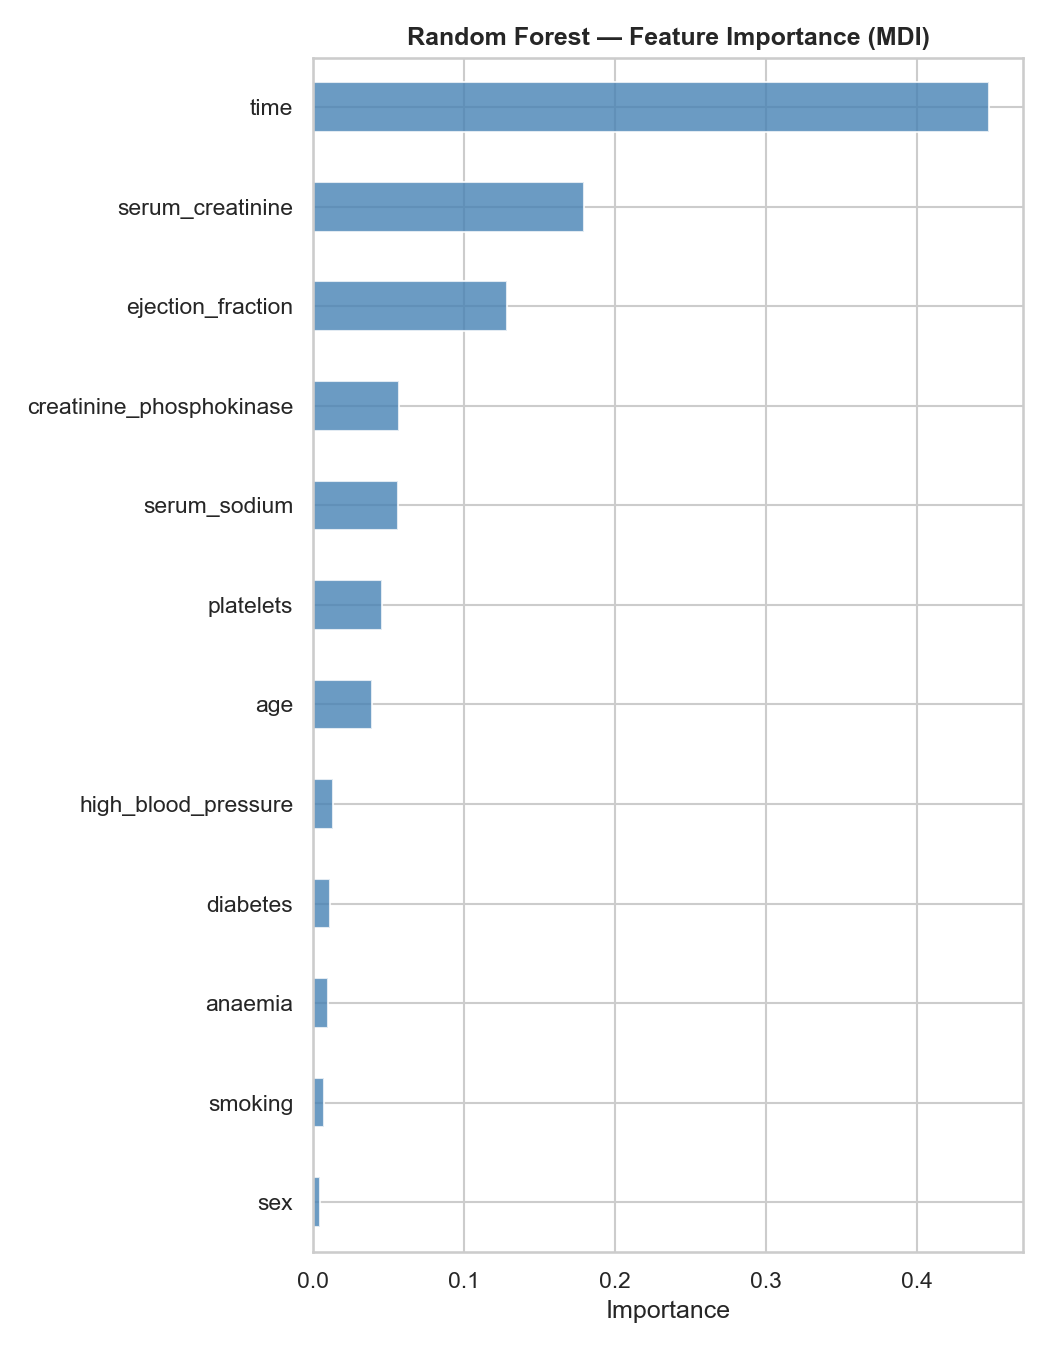
\includegraphics[width=\textwidth]{figures/feature_importance_rf.png}
\end{figure}

L'importanza MDI misura di quanto ogni feature riduce l'impurità media nei 200 alberi del Random
Forest: \texttt{time} domina nettamente, seguita da \texttt{serum\_creatinine} ed
\texttt{ejection\_fraction}. Questa gerarchia è confermata in modo indipendente da RuleFit
(sezione~3.4): le regole con coefficiente Lasso più alto coinvolgono \texttt{time} basso e
\texttt{serum\_creatinine} alta. Due metodi radicalmente diversi --- importance da ensemble di
alberi vs regressione Lasso su regole estratte --- convergono sugli stessi tre segnali
fisiopatologici, coerenti con la letteratura sull'insufficienza cardiaca.


\section{Conclusioni}

\subsection{Confronto, analisi clinica e limiti}

\textbf{Confronto tra approcci.}
I modelli ensemble raggiungono ROC-AUC superiore (Random Forest 0.896, XGBoost 0.843)
ma il divario con i rule-based non è netto: GreedyRuleList (0.833) è competitivo su un
dataset di soli 299 campioni, dove la semplicità strutturale riduce il rischio di overfitting.
GreedyRuleList offre il miglior F1 rule-based (0.667) con una lista ordinata di condizioni
leggibile da un clinico. RuleFit assegna coefficienti espliciti a ogni regola, rendendo visibile
il peso relativo di ciascuna. BayesianRuleList privilegia il recall (0.526): sovrastima i
decessi, il che in medicina è spesso preferibile a sottostimarli. FIGS ha struttura additiva
particolarmente trasparente. SkopeRules raggiunge Precision=1.0 con Recall molto basso: non
produce mai falsi positivi, ma identifica solo una piccola frazione dei deceduti --- utile quando
ogni allarme deve corrispondere a un caso critico. RIPPER è l'unico rule-list a produrre regole
congiuntive (AND tra più condizioni): nonostante la maggiore espressività strutturale, ottiene
il ROC-AUC più basso di tutti i modelli. Il vantaggio strutturale non si traduce in migliore
capacità discriminativa su questo dataset.

\medskip
\begin{center}
{\small\begin{tabular}{>{\raggedright\arraybackslash}p{0.3020\linewidth}>{\raggedright\arraybackslash}p{0.1954\linewidth}>{\raggedright\arraybackslash}p{0.1954\linewidth}>{\raggedright\arraybackslash}p{0.1954\linewidth}}
\toprule
\cellcolor{tblhdr}\color{white}\bfseries Modello & \cellcolor{tblhdr}\color{white}\bfseries Categoria & \cellcolor{tblhdr}\color{white}\bfseries ROC-AUC & \cellcolor{tblhdr}\color{white}\bfseries F1 \\
\midrule
SkopeRules & Rule-based & 0.8960 & 0.1000 \\
\rowcolor{ltrow}RandomForest & Ensemble & 0.8960 & 0.7500 \\
\bottomrule
\end{tabular}}}
\end{center}

\medskip
\textbf{Tuning degli iperparametri.}
La selezione sul validation set ha mostrato che per BayesianRuleList la cardinalità ottimale è
1 (regole a condizione singola sono sufficienti su questo dataset), mentre per SkopeRules
\texttt{max\_depth=2} produce regole bi-condizionali ad alta precisione. Per gli ensemble,
i valori ottimali tendono a configurazioni più semplici (meno stimatori, alberi poco profondi),
coerente con la dimensione ridotta del dataset.

\textbf{Precision vs Recall in ambito clinico.}
Il trade-off tra precisione e recall non è neutro in contesti medici. Alta recall minimizza i
falsi negativi (morti non rilevate), che in clinica sono più pericolosi dei falsi positivi
(falsi allarmi). Alta precisione garantisce invece che ogni segnalazione sia affidabile,
preferibile quando si pianificano interventi invasivi. La scelta del modello dipende quindi
dal contesto d'uso, e la trasparenza dei modelli rule-based è la condizione necessaria per
fare questa scelta in modo consapevole.

\textbf{Validazione qualitativa delle regole.}
Le feature più ricorrenti --- \texttt{time} (follow-up), \texttt{serum\_creatinine} ed
\texttt{ejection\_fraction} --- sono coerenti con la letteratura clinica sull'insufficienza
cardiaca: follow-up breve segnala una fase acuta critica, creatinina alta indica insufficienza
renale, ejection fraction bassa riflette ridotta capacità di pompa. Il fatto che i modelli
apprendano autonomamente queste relazioni costituisce una validazione qualitativa.

\textbf{Ablazione della feature \texttt{time}.}
Rimuovendo \texttt{time} da RF e GRL (con ri-tuning sul validation set senza \texttt{time}),
il ROC-AUC scende di circa 0.10 per entrambi i modelli. Senza \texttt{time} i modelli si
affidano a \texttt{serum\_creatinine} ed \texttt{ejection\_fraction} --- feature biochimiche
disponibili alla prima valutazione, prima del follow-up --- e rimangono utilizzabili in contesti
di triage, anche se con discriminazione ridotta.

\textbf{Limiti e sviluppi futuri.}
Con $\approx$60 campioni nel test set (circa 19 deceduti) ogni metrica è soggetta ad alta
varianza: un solo paziente classificato diversamente sposta F1 di oltre 0.05. I risultati
sono quindi indicativi e richiedono validazione su coorti esterne prima di qualsiasi
applicazione clinica. Ulteriori sviluppi potrebbero includere la calibrazione delle
probabilità predette e l'integrazione in un sistema di supporto decisionale con supervisione
medica --- contesto in cui la trasparenza dei modelli rule-based resta il requisito
imprescindibile.

\end{document}